% **************************************************************************************************************
% A Classic Thesis Style
% An Homage to The Elements of Typographic Style
%
% Copyright (C) 2012 Andr\'e Miede http://www.miede.de
%
% If you like the style then I would appreciate a postcard. My address 
% can be found in the file ClassicThesis.pdf. A collection of the 
% postcards I received so far is available online at 
% http://postcards.miede.de
%
% License:
% This program is free software; you can redistribute it and/or modify
% it under the terms of the GNU General Public License as published by
% the Free Software Foundation; either version 2 of the License, or
% (at your option) any later version.
%
% This program is distributed in the hope that it will be useful,
% but WITHOUT ANY WARRANTY; without even the implied warranty of
% MERCHANTABILITY or FITNESS FOR A PARTICULAR PURPOSE.  See the
% GNU General Public License for more details.
%
% You should have received a copy of the GNU General Public License
% along with this program; see the file COPYING.  If not, write to
% the Free Software Foundation, Inc., 59 Temple Place - Suite 330,
% Boston, MA 02111-1307, USA.
%
% **************************************************************************************************************
% Note:
%    * You must not use "u etc. in strings/commands that will be spaced out (use \"u or real umlauts instead)
%    * New enumeration (small caps): \begin{aenumerate} \end{aenumerate}
%    * For margin notes: \marginpar or \graffito{}
%    * Do not use bold fonts in this style, it is designed around them
%    * Use tables as in the examples
%    * See classicthesis-preamble.sty for useful commands
% **************************************************************************************************************
% To Do:
%   * [high] Check this out: http://www.golatex.de/koma-script-warnung-in-verbindung-mit-listings-package-t2058.html
%   * [medium] mathbb in section-titles/chapter-titles => disappears somehow in headlines!!!
% **************************************************************************************************************
\documentclass[
  twoside,
  openright,
  titlepage,
  numbers=noenddot,
  headinclude,
  footinclude=true,
  cleardoublepage=plain,
  abstract=false,  % Modern replacement for abstractoff
  BCOR=5mm,
  paper=a4,
  fontsize=11pt,
  english,ngerman,portuguese,
  dottedtoc,
]{scrreprt}


% UTF-8 support with latin9 (ISO-8859-9) = latin1+"Euro sign"
\PassOptionsToPackage{utf8}{inputenc}   
\usepackage[utf8]{inputenc} % For UTF-8 support
 
% ****************************************************************************************************
% Personal data and user ad-hoc commands
% ****************************************************************************************************
\newcommand{\myTitle}{BattAIHealth \\ Battery Condition Estimation in
Automotive and Railway Applications using AI\xspace}
\newcommand{\myDegree}{Bachelor's Degree in Electrical and Computer Engineering\xspace}

\newcommand{\myNameOne}{Pedro André Silva Ferreira\xspace}
\newcommand{\myNumber}{2222035}

\newcommand{\myProfOne}{Professor Lu\'{i}s Conde Bento}
\newcommand{\myProfTwo}{Professor M\'{o}nica Figueiredo}
\newcommand{\ProfLuisEmail}{\href{mailto:luis.conde@ipleiria.pt}{\texttt{(luis.conde@ipleiria.pt)}}}
\newcommand{\ProfMonicaEmail}{\href{mailto:monica.figueiredo@ipleiria.pt}{\texttt{(monica.figueiredo@ipleiria.pt)}}}

\newcommand{\myFaculty}{Polytechnic of Leiria\xspace}
\newcommand{\mySchool}{School of Technology and Management\xspace}
\newcommand{\myDepartment}{Department of Electrical Engineering\xspace}

\newcommand{\myLocation}{Leiria\xspace}

\newcommand{\myTime}{Junho de 2025\xspace}
\newcommand{\mySchoolYear}{2024 -- 2025\xspace}
\newcommand{\myVersion}{versão 0.1\xspace}            
                
                
%*******************************************************
% Note: Make all your adjustments in here
%*******************************************************
% ****************************************************************************************************
% classicthesis-config.tex 
% formerly known as loadpackages.sty, classicthesis-ldpkg.sty, and classicthesis-preamble.sty 
% Use it at the beginning of your ClassicThesis.tex, or as a LaTeX Preamble 
% in your ClassicThesis.{tex,lyx} with \input{classicthesis-config}
% ****************************************************************************************************  
% If you like the classicthesis, then I would appreciate a postcard. 
% My address can be found in the file ClassicThesis.pdf. A collection 
% of the postcards I received so far is available online at 
% http://postcards.miede.de
% ****************************************************************************************************

% ****************************************************************************************************
% 1. Configure classicthesis for your needs here, e.g., remove "drafting" below 
% in order to deactivate the time-stamp on the pages
% ****************************************************************************************************
\PassOptionsToPackage{
                    eulerchapternumbers,
%                    drafting, % comentar para remover a linha com a versão
                    pdfspacing,
                    %floatperchapter,
                    %linedheaders,%
                    subfig,beramono,
%                    eulermath,
                    parts
                    }{classicthesis}
% Available options for classicthesis.sty 
% (see ClassicThesis.pdf for more information):
% drafting
% parts nochapters linedheaders
% eulerchapternumbers beramono eulermath pdfspacing minionprospacing
% tocaligned dottedtoc manychapters
% listings floatperchapter subfig
% ********************************************************************

% ********************************************************************
% Triggers for this config
% ******************************************************************** 
\usepackage{ifthen}
\newboolean{enable-backrefs} % enable backrefs in the bibliography
\setboolean{enable-backrefs}{false} % true false
% ****************************************************************************************************


% ********************************************************************
% Setup, finetuning, and useful commands
% ********************************************************************
\newcounter{dummy} % necessary for correct hyperlinks (to index, bib, etc.)
\newlength{\abcd} % for ab..z string length calculation
\providecommand{\mLyX}{L\kern-.1667em\lower.25em\hbox{Y}\kern-.125emX\@}
\newcommand{\ie}{\textit{i.\,e.}\xspace}
\newcommand{\Ie}{\textit{I.\,e.}\xspace}
\newcommand{\eg}{\textit{e.\,g.}\xspace}
\newcommand{\Eg}{\textit{E.\,g.}\xspace} 
\newcommand{\etc}{\textit{etc}\xspace} 


% ****************************************************************************************************
% \DeclareTextFontCommand{\code}{\fontfamily{pcr}\scriptsize}


% ****************************************************************************************************
% 3. Loading some handy packages
% ****************************************************************************************************
% ******************************************************************** 
% Packages with options that might require adjustments
% ******************************************************************** 

\PassOptionsToPackage{portuguese}{babel}
\usepackage{babel}

 
%%%%%%%%%%%%%%%%%%%%%%%%%%%%%%%%%%%%%%%%%%%%%%%%%%%%%
% Bibliografia
%%%%%%%%%%%%%%%%%%%%%%%%%%%%%%%%%%%%%%%%%%%%%%%%%%%%%
% package recomendada para usar com o biblatex
\usepackage{csquotes}

% carrega a package biblatex
\usepackage[
    backend=biber,    % usar o biber para processar
    style=numeric,    % estilo de citação numérica
    sortcites=true,
    maxcitenames=2,   % a partir de 2 escreve "et al."
]{biblatex} 

% Remove the period after citation numbers
\DeclareFieldFormat{labelnumberwidth}{#1}

% para adicionar uma vírgula antes do ano: (Dirac, 1981)
\renewcommand*{\nameyeardelim}{\addcomma\space}

%  dica: configurar o kile para reconhecer os comandos:
%    \parencite{bibkey}
%    \textcite{bibkey}
%    \citeauthor{bibkey}
%    \citetitle{bibkey}
%    
%    Settingis -> Configure Kile -> Latex/General -> Commands/Configure -> Commands/Citation -> add
%%%%%%%%%%%%%%%%%%%%%%%%%%%%%%%%%%%%%%%%%%%%%%%%%%%%%
 
\usepackage{float}

\PassOptionsToPackage{fleqn}{amsmath}		% math environments and more by the AMS 
\usepackage{amsmath}
\usepackage{amsfonts}                       % AMS fonts
\usepackage{amssymb}                        % AMS symbols
\usepackage{mathtools}                      % Enhanced math tools

\usepackage{multirow}
 
%******************************************************************** 
% General useful packages
%******************************************************************** 
\PassOptionsToPackage{T1}{fontenc} % T2A for cyrillics
\usepackage{fontenc}

\usepackage{textcomp} % fix warning with missing font shapes
\usepackage{scrhack} % fix warnings when using KOMA with listings package          
\usepackage{xspace} % to get the spacing after macros right  
\usepackage{mparhack} % get marginpar right
% \usepackage{fixltx2e} % fixes some LaTeX stuff 

% \PassOptionsToPackage{printonlyused,smaller}{acronym}
% \usepackage[acronym,toc]{glossaries} % nice macros for handling all acronyms in the thesis
% \makeglossaries % Enable glossary generation

%\renewcommand*{\acsfont}[1]{\textssc{#1}} % for MinionPro
\newcommand{\bflabel}[1]{{#1}\hfill} % fix the list of acronyms
%****************************************************************************************************


%****************************************************************************************************
% 4. Setup floats: tables, (sub)figures, and captions
%****************************************************************************************************
\usepackage{tabularx} % better tables
    \setlength{\extrarowheight}{3pt} % increase table row height
\newcommand{\tableheadline}[1]{\multicolumn{1}{c}{\spacedlowsmallcaps{#1}}}
\newcommand{\tableheadlineR}[1]{\multicolumn{1}{r}{\spacedlowsmallcaps{#1}}}
\newcommand{\myfloatalign}{\centering} % to be used with each float for alignment
\usepackage{caption}
\captionsetup{format=hang,font=small}
\usepackage{subfig}  
% ****************************************************************************************************


%----------------------------------------------------------
% Filipius's famous "issue" command (Patricio, 2016-08-03)
%----------------------------------------------------------
\newcommand{\issue}[1] { {\footnotesize\textbf{
    \begin{center}
      \begin{tabular}{|c|}
        \hline
	\parbox[c]{\textwidth}{
          \medskip
          #1
          \medskip} \\
        \hline
      \end{tabular}
    \end{center}
  }
 }
}


% ****************************************************************************************************
% 6. PDFLaTeX, hyperreferences and citation backreferences
% ****************************************************************************************************
% ********************************************************************
% Using PDFLaTeX
% ********************************************************************
\PassOptionsToPackage{pdftex,hyperfootnotes=false,pdfpagelabels}{hyperref}
	\usepackage{hyperref}  % backref linktocpage pagebackref
\pdfcompresslevel=9
\pdfadjustspacing=1 
\PassOptionsToPackage{pdftex}{graphicx}
	\usepackage{graphicx} 

% ********************************************************************
% Setup the style of the backrefs from the bibliography
% (translate the options to any language you use)
% ********************************************************************
\newcommand{\backrefnotcitedstring}{\relax}%(Not cited.)
\newcommand{\backrefcitedsinglestring}[1]{(Cited on page~#1.)}
\newcommand{\backrefcitedmultistring}[1]{(Cited on pages~#1.)}
\ifthenelse{\boolean{enable-backrefs}}%
{%
		\PassOptionsToPackage{hyperpageref}{backref}
		\usepackage{backref} % to be loaded after hyperref package 
		   \renewcommand{\backreftwosep}{ and~} % separate 2 pages
		   \renewcommand{\backreflastsep}{, and~} % separate last of longer list
		   \renewcommand*{\backref}[1]{}  % disable standard
		   \renewcommand*{\backrefalt}[4]{% detailed backref
		      \ifcase #1 %
		         \backrefnotcitedstring%
		      \or%
		         \backrefcitedsinglestring{#2}%
		      \else%
		         \backrefcitedmultistring{#2}%
		      \fi}%
}{\relax}    

% ********************************************************************
% Hyperreferences
% ********************************************************************
\hypersetup{%
    %draft,	% = no hyperlinking at all (useful in b/w printouts)
    colorlinks=true, linktocpage=true, pdfstartpage=3, pdfstartview=FitV,%
    % uncomment the following line if you want to have black links (e.g., for printing)
    %colorlinks=false, linktocpage=false, pdfborder={0 0 0}, pdfstartpage=3, pdfstartview=FitV,% 
    breaklinks=true, pdfpagemode=UseNone, pageanchor=true, pdfpagemode=UseOutlines,%
    plainpages=false, bookmarksnumbered, bookmarksopen=true, bookmarksopenlevel=1,%
    hypertexnames=true, pdfhighlight=/O,%nesting=true,%frenchlinks,%
    urlcolor=RoyalBlue, linkcolor=RoyalBlue, citecolor=RoyalBlue, %pagecolor=RoyalBlue,%
    %urlcolor=Black, linkcolor=Black, citecolor=Black, %pagecolor=Black,%
    pdftitle={\myTitle},%
    pdfauthor={\textcopyright\ \myNameOne, \myDegree, \myDepartment, \mySchool, \myFaculty},%
    pdfsubject={},%
    pdfkeywords={},%
    pdfcreator={pdfLaTeX},%
    pdfproducer={LaTeX with hyperref and classicthesis}%
}   

% ********************************************************************
% Setup autoreferences
% ********************************************************************
% There are some issues regarding autorefnames
% http://www.ureader.de/msg/136221647.aspx
% http://www.tex.ac.uk/cgi-bin/texfaq2html?label=latexwords
% you have to redefine the makros for the 
% language you use, e.g., american, ngerman
% (as chosen when loading babel/AtBeginDocument)
% ********************************************************************
\makeatletter
\@ifpackageloaded{babel}%
    {%
       \addto\extrasamerican{%
					\renewcommand*{\figureautorefname}{Figure}%
					\renewcommand*{\tableautorefname}{Table}%
					\renewcommand*{\partautorefname}{Part}%
					\renewcommand*{\chapterautorefname}{Chapter}%
					\renewcommand*{\sectionautorefname}{Section}%
					\renewcommand*{\subsectionautorefname}{Section}%
					\renewcommand*{\subsubsectionautorefname}{Section}% 	
				}%
       \addto\extrasngerman{% 
					\renewcommand*{\paragraphautorefname}{Absatz}%
					\renewcommand*{\subparagraphautorefname}{Unterabsatz}%
					\renewcommand*{\footnoteautorefname}{Fu\"snote}%
					\renewcommand*{\FancyVerbLineautorefname}{Zeile}%
					\renewcommand*{\theoremautorefname}{Theorem}%
					\renewcommand*{\appendixautorefname}{Anhang}%
					\renewcommand*{\equationautorefname}{Gleichung}%        
					\renewcommand*{\itemautorefname}{Punkt}%
				}%	
			% Fix to getting autorefs for subfigures right (thanks to Belinda Vogt for changing the definition)
			\providecommand{\subfigureautorefname}{\figureautorefname}%  			
    }{\relax}
\makeatother


% ****************************************************************************************************
% 7. Last calls before the bar closes
% ****************************************************************************************************
% ********************************************************************
% Development Stuff
% ********************************************************************
\listfiles
%\PassOptionsToPackage{l2tabu,orthodox,abort}{nag}
%	\usepackage{nag}
%\PassOptionsToPackage{warning, all}{onlyamsmath}
%	\usepackage{onlyamsmath}


% ********************************************************************
% Last, but not least...
% ********************************************************************
\usepackage{classicthesis} 
% ****************************************************************************************************


\clearpairofpagestyles
\ohead[]{\headmark}
\ofoot[\pagemark]{\pagemark}

% incluir PDFs
\usepackage{pdfpages}

% ****************************************************************************************************
% 8. Further adjustments (experimental)
% ****************************************************************************************************

\usepackage{setspace}

% recomendado por ser o mais próximo do word
\spacing{1.3}


% ********************************************************************
% Changing the text area
% ********************************************************************
%\linespread{1.05} % a bit more for Palatino
%\areaset[current]{312pt}{761pt} % 686 (factor 2.2) + 33 head + 42 head \the\footskip
%\setlength{\marginparwidth}{7em}%
%\setlength{\marginparsep}{2em}%

% ********************************************************************
% Using different fonts
% ********************************************************************
%\usepackage[oldstylenums]{kpfonts} % oldstyle notextcomp
%\usepackage[osf]{libertine}
%\usepackage{hfoldsty} % Computer Modern with osf
%\usepackage[light,condensed,math]{iwona}
%\renewcommand{\sfdefault}{iwona}
\usepackage{lmodern} % <-- no osf support :-(
%\usepackage[urw-garamond]{mathdesign} <-- no osf support :-(
% ****************************************************************************************************

% \usepackage{inconsolata}

\usepackage{caption}
% \usepackage{caption,setspace}
% \captionsetup[lstlisting]{belowskip=0pt}
% \captionsetup[lstlisting]{belowcaptionskip=0pt}
% \captionsetup[lstinputlisting]{belowcaptionskip=0pt}
% \captionsetup[listing]{font={stretch=0.8}}


% o mint dá erro se pedirmos para imprimir o @
\newcommand{\at}{\makeatletter @\makeatother}



% controlar o tamanho das margens
% \usepackage{showframe}
\marginparwidth=0pt
\marginparsep=5pt
\addtolength{\evensidemargin}{-15mm}
\addtolength{\textwidth}{20mm}

% espaçamento entre parágrafos
\setlength{\parskip}{0.5em}

% obter o símbolo do Euro
\usepackage{eurosym}
\DeclareUnicodeCharacter{20AC}{\euro} % aceita o símbolo do teclado
% usar a vírgula como separador decimal
\usepackage{icomma}

% 
% tem de ser carregada depois do hyperref
% 
\PassOptionsToPackage{xindy,style=super}{glossaries}
\PassOptionsToPackage{acronym}{glossaries}
\PassOptionsToPackage{nonumberlist}{glossaries}
\usepackage{glossaries}


% avoid numbering empty pages
\usepackage{emptypage}


% permite quebrar a 1ª coluna - COMMENTED OUT (using manual acronym list)
% \newglossarystyle{clong}{%
%  \renewenvironment{theglossary}%
% %      {\begin{longtable}{p{.2\linewidth}p{\glsdescwidth}}}%
%      {\begin{longtable}{p{.18\linewidth}p{.78\linewidth}}}%
%      {\end{longtable}}%
%   \renewcommand*{\glossaryheader}{}%
%   \renewcommand*{\glsgroupheading}[1]{}%
%   \renewcommand*{\glossaryentryfield}[5]{%
%     \glstarget{##1}{##2} & ##3\glspostdescription\space ##5\\}%
%   \renewcommand*{\glossarysubentryfield}[6]{%
%      & \glstarget{##2}{\strut}##4\glspostdescription\space ##6\\}%
%   %\renewcommand*{\glsgroupskip}{ & \\}%
% }

\usepackage{lipsum}
\usepackage{amsmath}
\usepackage{geometry}
\usepackage{amsfonts} % For \mathbb, \mathfrak, etc.
\usepackage{amssymb}  % For extra symbols
\usepackage{mathtools} % Extends amsmath



%*******************************************************
% Bibliography
%*******************************************************
%   Ficheiro com a base de dados da bibliografia
\addbibresource{References.bib}
%   para o kile dar as sugestões das chaves da bibliografia
%   se der erro a queixar-se do bibtex, basta repetir a compilação
\iffalse
    \bibliography{References.bib}  % só para o kile
\fi


%*******************************************************
% Lista de acrónimos
%*******************************************************
% GLOSSARIES ACRONYM DEFINITIONS COMMENTED OUT - Using simple static list instead
% \loadglsentries{Covers/Acronyms-list}

% Load acronym definitions
% \newacronym{cnn}{CNN}{Convolutional Neural Network}
% \newacronym{efk}{EKF}{Extended Kalman Filter}
% \newacronym{lstm}{LSTM}{Long Short-Term Memory}
% \newacronym{soc}{SoC}{State of Charge}
% \newacronym{soh}{SoH}{State of Health}

% \makeglossaries  % Commented out - already defined in config.tex


%*******************************************************
% Hyphenation
%*******************************************************
%\hyphenation{put special hyphenation here}


% ******************************************************
% GO!GO!GO! MOVE IT!
%*******************************************************
\begin{document}
\frenchspacing
\raggedbottom
%\selectlanguage{portuguese}
\selectlanguage{English}
\pagestyle{plain}

% use \cleardoublepage here to avoid problems with pdfbookmark

%*******************************************************
% Frontmatter
%*******************************************************
% Title Page

\begin{titlepage}

\begin{center}
\large

\hfill

% \includegraphics[width=8cm]{Covers/ipl-estg} \\

\includegraphics[width=\textwidth]{Covers/estg_h.pdf} \\


\bigskip
\myFaculty \\
\mySchool \\ 
\myDepartment \\
\myDegree \\



\begingroup
\color{Maroon}

\vspace{4cm}

\spacedallcaps{\myTitle} \\ \bigskip % Thesis title
\endgroup
% \mySubtitle \\ \medskip % Thesis subtitle

\vspace{4cm}

% \vfill


\spacedlowsmallcaps{\myNameOne} \\
% \spacedlowsmallcaps{\myNameTwo}
\bigskip % Your name

\vfill


\myLocation, \myTime\ %-- \myVersion % Time and version



\end{center}
% \end{addmargin}

\end{titlepage}


\cleardoublepage% Title Page

\begin{titlepage}

\begin{center}

\hfill

% \includegraphics[width=8cm]{Covers/ipl-estg} \\

\includegraphics[width=\textwidth]{Covers/estg_h.pdf} \\

\bigskip
\large
\myFaculty \\
\mySchool \\ 
\myDepartment \\
\myDegree \\



\begingroup
\color{Maroon}

\vspace{2cm}

\spacedallcaps{\myTitle} \\ \bigskip % Thesis title
\endgroup
% \mySubtitle \\ \medskip % Thesis subtitle

\vspace{1cm}

% \vfill

\noindent Final report of the Project Curricular Unit of the Bachelor’s Degree in Eletrotechnical and Computers Engineering, branch of Eletronics and Computers.

\vspace{1cm}

\spacedlowsmallcaps{\myNameOne}\\
N: \myNumber \\
% \spacedlowsmallcaps{\myNameTwo}
\bigskip % Your name

\vfill

\end{center}

\begin{normalsize}
    
\noindent Work done under the guidance of \myProfOne \ProfLuisEmail and \myProfTwo \ProfMonicaEmail.

\end{normalsize}
\vspace{1cm}

\begin{center}

\myLocation, \myTime\ %-- \myVersion % Time and version
    
\end{center}



% \end{addmargin}

\end{titlepage}

\cleardoublepage

\pagenumbering{roman}
\cleardoublepage%*******************************************************
% Acknowledgments
%*******************************************************


\refstepcounter{dummy}
\addcontentsline{toc}{chapter}{Acknowledgements}

% \begin{flushright}{\slshape    
%     We have seen that computer programming is an art, \\ 
%     because it applies accumulated knowledge to the world, \\ 
%     because it requires skill and ingenuity, and especially \\
%     because it produces objects of beauty.} \\ \medskip
%     --- Donald Knuth
% \end{flushright}
% 
% 
% 
% \bigskip

\begingroup
\let\clearpage\relax
\let\cleardoublepage\relax
\let\cleardoublepage\relax
\chapter*{Acknowledgements}
I would like to express my deepest gratitude to those who have supported me throughout this journey. To my girlfriend, mother, father, brother, and family, thank you for your unwavering support, encouragement, and love over the years. Your presence has been a constant source of strength and inspiration.

I am profoundly grateful to my supervisors, Professor Luís Conde Bento and Professor Mónica Figueiredo, for their invaluable guidance and expertise. They introduced me to an entirely new field of study, broadening my knowledge and teaching me innovative methods of work that have shaped my academic and professional growth.

Finally, I extend my heartfelt thanks to my friends who have been by my side since the beginning of this course. Their companionship, encouragement, and shared experiences have been instrumental in keeping me motivated and focused throughout this work.

\endgroup



%\cleardoublepage%----------------------------------------------------------------------------------------
%   Resumo (Portuguese Abstract)
%----------------------------------------------------------------------------------------

\selectlanguage{portuguese}
\pdfbookmark[1]{Resumo}{Resumo}
\chapter*{Resumo}

% Add your Portuguese abstract content here
Este trabalho apresenta um estudo sobre a estimação da condição de baterias em aplicações automotivas e ferroviárias utilizando inteligência artificial. O projeto foca na monitorização da saúde de baterias através de parâmetros como Estado de Carga (SoC), Estado de Saúde (SoH) e Vida Útil Remanescente (RUL). Utilizando técnicas de aprendizagem automática e análise de séries temporais, desenvolvemos modelos preditivos capazes de identificar padrões de degradação e prever falhas em sistemas de baterias. Os resultados demonstram a eficácia das abordagens baseadas em IA para melhorar a confiabilidade e segurança dos sistemas de energia em aplicações críticas.

\vfill

\noindent
\textbf{Palavras-chave:} Inteligência Artificial, Baterias, Estado de Saúde, Monitorização, Aprendizagem Automática

\selectlanguage{English}

\cleardoublepage%*******************************************************
% Abstract
%*******************************************************


\renewcommand{\abstractname}{Resumo}
\markboth{\spacedlowsmallcaps{\abstractname}}{\spacedlowsmallcaps{\abstractname}}
\refstepcounter{dummy}
\addcontentsline{toc}{chapter}{\abstractname}


\begingroup
\let\clearpage\relax
\let\cleardoublepage\relax
\let\cleardoublepage\relax

\chapter*{Resumo}
Deverá conter de forma sucinta, clara e objetiva as questões mais importantes tratadas no corpo do trabalho.\newline
Deverá ter, no máximo, 250 palavras.\\

\bigskip

\endgroup			

\cleardoublepage

\renewcommand{\abstractname}{Abstract}
\markboth{\spacedlowsmallcaps{\abstractname}}{\spacedlowsmallcaps{\abstractname}}
\refstepcounter{dummy}
\addcontentsline{toc}{chapter}{\abstractname}


\begingroup
\let\clearpage\relax
\let\cleardoublepage\relax
\let\cleardoublepage\relax

\chapter*{Abstract}
Escrever o resumo em inglês.\\

\bigskip


\endgroup           

\pagestyle{scrheadings}

\cleardoublepage% Table of Contents - List of Tables/Figures/Listings and Acronyms

\refstepcounter{dummy}

% \addcontentsline{toc}{chapter}{Índice}
% \pdfbookmark[1]{\contentsname}{tableofcontents} % Bookmark name visible in a PDF viewer

\setcounter{tocdepth}{2} % Depth of sections to include in the table of contents - currently up to subsections

\setcounter{secnumdepth}{3} % Depth of sections to number in the text itself - currently up to subsubsections

\renewcommand\contentsname{Index}

\manualmark
\markboth{\spacedlowsmallcaps{\contentsname}}{\spacedlowsmallcaps{\contentsname}}
\tableofcontents 
\automark[section]{chapter}
\renewcommand{\chaptermark}[1]{\markboth{\spacedlowsmallcaps{#1}}{\spacedlowsmallcaps{#1}}}
\renewcommand{\sectionmark}[1]{\markright{\thesection\enspace\spacedlowsmallcaps{#1}}}

% \clearpage

\vspace*{8ex}
\newpage
\cleardoublepage

% \begingroup 
% \let\clearpage\relax
% \let\cleardoublepage\relax
% \let\cleardoublepage\relax

%----------------------------------------------------------------------------------------
%	List of Figures
%----------------------------------------------------------------------------------------

\refstepcounter{dummy}
\addcontentsline{toc}{chapter}{\listfigurename} % Uncomment if you would like the list of figures to appear in the table of contents
% \pdfbookmark[1]{\listfigurename}{lof} % Bookmark name visible in a PDF viewer

\listoffigures

\vspace*{8ex}
% \newpage
\cleardoublepage

%----------------------------------------------------------------------------------------
%	List of Tables
%----------------------------------------------------------------------------------------

% \phantomsection 
\refstepcounter{dummy}
\addcontentsline{toc}{chapter}{\listtablename} % Uncomment if you would like the list of tables to appear in the table of contents
% \pdfbookmark[1]{\listtablename}{lot} % Bookmark name visible in a PDF viewer

\listoftables

\clearpage

\vspace*{8ex}
% \newpage
% \cleardoublepage
    
%----------------------------------------------------------------------------------------
%	List of Listings
%---------------------------------------------------------------------------------------- 

% \refstepcounter{dummy}
% %\addcontentsline{toc}{chapter}{\lstlistlistingname} % Uncomment if you would like the list of listings to appear in the table of contents
% \pdfbookmark[1]{\lstlistlistingname}{lol} % Bookmark name visible in a PDF viewer
% 
% % \lstlistoflistings 
% 
% \vspace*{8ex}
% \newpage
       
% \endgroup



% %----------------------------------------------------------------------------------------
% %	Glossário
% %----------------------------------------------------------------------------------------
% 
% 
% \refstepcounter{dummy}
% \addcontentsline{toc}{chapter}{Glossary} % Uncomment if you would like the acronyms to appear in the table of contents
% \pdfbookmark[1]{List of Acronyms}{List of Acronyms} % Bookmark name visible in a PDF viewer
% 
% 
% 
% \markboth{\spacedlowsmallcaps{Glossary}}{\spacedlowsmallcaps{Glossary}}
% \printglossary[type=\glsdefaulttype,title=Glossary]
 
 
 
 
 \cleardoublepage
\cleardoublepage%----------------------------------------------------------------------------------------
%   LIST OF ACRONYMS
%----------------------------------------------------------------------------------------

\cleardoublepage
\phantomsection
\addcontentsline{toc}{chapter}{List of Acronyms}

\chapter*{LIST OF ACRONYMS}

\begin{description}
    \item[AI] Artificial Intelligence
    \item[BMS] Battery Management System
    \item[CALCE] Center for Advanced Life Cycle Engineering
    \item[CNN] Convolutional Neural Network
    \item[DAE] Denoising Auto-Encoder
    \item[ECM] Equivalent Circuit Model
    \item[EFK] Extended Kalman Filter
    \item[FFT] Fast Fourier Transform
    \item[LFP] Lithium Iron Phosphate
    \item[LSTM] Long Short-Term Memory
    \item[MAE] Mean Absolute Error
    \item[MAPE] Mean Absolute Percentage Error
    \item[ML] Machine Learning
    \item[MoE] Mixture of Experts
    \item[MSE] Mean Squared Error
    \item[NN] Neural Network
    \item[PE] Positive Electrode
    \item[RMSE] Root Mean Squared Error
    \item[RNN] Recurrent Neural Network
    \item[RUL] Remaining Useful Life
    \item[SEI] Solid Electrolyte Interphase
    \item[SOC] State of Charge
    \item[SOH] State of Health
    \item[SVM] Support Vector Machine
    \item[TPE] Tree-structured Parzen Estimator
    \item[WandB] Weights and Biases
\end{description}

\cleardoublepage



%********************************************************************
% Mainmatter
%*******************************************************
\pagenumbering{arabic}

% \phantomsection 
% \part*{Relatório}


\cleardoublepage\addtocontents{toc}{\protect\vspace{\beforebibskip}} % Place slightly below the rest of the document content in the table

%************************************************
\chapter{Introduction}
\label{ch:introduction}
%************************************************

Electric vehicles and electrified trains rely on accurate battery health monitoring to ensure safety and reliability. This involves keeping track of three key parameters: SOC, which reflects the remaining energy; SOH, which indicates how much the battery has degraded over time; and RUL, which estimates how much longer the battery can operate. Predicting these parameters is challenging because batteries undergo complex chemical processes that change with temperature, usage patterns, and aging.

Traditional methods like coulomb counting and Kalman filters have their limits, they perform reasonably well in controlled environments, but struggle in real-world conditions where temperatures and loads vary, and where aging causes nonlinear behavior.

Most current battery management systems still use decades old techniques that don’t adapt well to the way batteries actually behave as they age, often leading to accumulating measurement errors over time.

Machine learning opens up new possibilities by uncovering patterns in battery data that traditional methods tend to miss. However, applying ML to battery health estimation comes with its own challenges: the models must work in real-time, handle different battery chemistries, and run on the limited computing power available in vehicles.

The main goal of this work is to develop methods that can predict SOC, SOH, and RUL simultaneously and accurately. This is difficult because each parameter behaves differently: SOC can change quickly during charge and discharge cycles, SOH declines slowly over months or years, and RUL depends both on the current condition of the battery and on how it will be used in the future.

This work contributes by comparing traditional and AI-based approaches, highlighting their strengths and weaknesses under realistic conditions. We also adapt the TimesNet architecture for battery data, leveraging its ability to capture periodic patterns and transform time series for better prediction. Along the way, we explore important trade-offs that arise when trying to predict multiple battery parameters at once.

The rest of this report is organized as follows: Chapter 2 covers background topics, including battery fundamentals, time series analysis, and evaluation metrics. Chapter 3 reviews existing battery health estimation methods, from traditional physics-based models to modern neural networks, and discusses available datasets. Chapter 4 describes our development process, from MATLAB-based modeling through different neural network architectures to our final TimesNet implementation. Chapter 5 presents experimental results, performance analysis, and comparisons with baseline methods, along with a discussion of limitations and challenges. Finally, Chapter 6 summarizes the key findings and offers recommendations for future research.

\cleardoublepage%************************************************
\chapter{Background Material and Supporting Technologies}
\label{ch:background}
%***********************************************

This chapter presents the basic background material and supporting tools that were used in the project. The first section covers the main ideas for battery health monitoring, including explanations of key battery parameters such as State of Charge (SoC), State of Health (SoH), and Remaining Useful Life (RUL). Also, the work covers the basic evaluation metrics used to check model performance and provides a discussion of battery wear mechanisms, that directly affect health estimation accuracy. The chapter also looks at the technical challenges in battery health monitoring, from the complexity of chemical processes to the difficulties of real-world use. Finally, it summarizes the software tools and platforms that supported the research and development process, from parameter tuning and experiment tracking to data display and version control.

\section{Core Concepts}

This section covers the main ideas basic to battery health monitoring, including detailed explanations of key battery parameters, evaluation metrics, wear mechanisms, and technical challenges. Battery technology serves as the foundation for energy storage systems across many applications. Modern batteries mainly fall into lithium-ion, lead-acid, nickel-metal hydride, and flow batteries, each with different chemical properties, energy densities, and lifecycle characteristics. The health of these batteries is shown by parameters such as state of charge (SoC), state of health (SoH), capacity fade, internal resistance, and wear rates, which together determine performance and longevity ~\cite{vijaychandra_comprehensive_2024}. Monitoring these parameters presents unique challenges due to the complex, nonlinear relationships between observable measurements and battery conditions. Artificial intelligence and machine learning approaches offer good solutions to these challenges by enabling pattern recognition across multidimensional battery data. Deep learning architectures, particularly recurrent neural networks and transformers, have shown exceptional ability in extracting temporal patterns from battery operational data, making them especially valuable for health prediction in dynamic usage scenarios~\cite{renold_comprehensive_2024}. 

%Battery fundamentals (types, chemistry, operating principles)
%Key health monitoring parameters for batteries
%AI/ML fundamentals relevant to your application

The following subsections provide detailed coverage of the fundamental concepts essential for understanding battery health monitoring and AI-based estimation methods. We begin with \textbf{time series analysis} and \textbf{spectral analysis} techniques that are crucial for processing battery operational data and extracting meaningful patterns from temporal sequences. The \textbf{evaluation metrics} section defines both battery-specific parameters (SoC, SoH, RUL) and machine learning performance measures (MAE, MSE, RMSE, MAPE) used throughout this work. \textbf{Neural networks and deep learning fundamentals} establish the theoretical foundation for the AI methods employed, while the \textbf{battery degradation and aging} section explains the physical mechanisms that drive battery health decline. Finally, we discuss the \textbf{challenges of battery health monitoring} that motivate the need for advanced AI approaches, and conclude with the \textbf{supporting technologies} that enabled this research.

\subsection{Time Series Analysis of Battery Data}

Time series analysis studies how battery parameters like voltage, current, and SoC change over time\cite{jorge_time_2023}. It helps model and predict battery behavior, find trends, and detect problems in the time domain. Time series analysis breaks down battery data into three basic parts that show different patterns in battery behavior and wear:

\begin{enumerate}
    \item \textbf{Trend Component} shows the long-term direction of battery parameters over time, capturing how the battery wears down and reflects basic changes in battery chemistry and structure. In battery health monitoring, trend analysis shows capacity loss patterns, where SoH slowly decreases over hundreds or thousands of charge-discharge cycles due to the wear mechanisms detailed in Section~\ref{sec:degradation}. The trend component is useful for RUL prediction, as it shows the rate of wear and helps set expected levels for battery performance decline under specific use conditions.
   \item  \textbf{Seasonal/Cyclic Component} finds repeated patterns that happen at regular times in battery data, showing periodic effects like daily use cycles, temperature changes, or charging schedules. In car applications, seasonal patterns may show as daily driving patterns that affect SoC changes, while in fixed energy storage systems, seasonal parts often match daily energy demand cycles or seasonal temperature changes that affect battery efficiency and capacity. These cyclic patterns are important for understanding how outside factors affect battery behavior and for building models that can handle predictable changes in performance.
   \item \textbf{Irregular/Noise Component} includes random changes and unpredictable variations that cannot be linked to trend or seasonal patterns, including measurement noise, sudden load changes, and random environmental factors. In battery monitoring systems, irregular parts may come from sensor limits, electrical interference, sudden acceleration events in vehicles, or unexpected temperature spikes. While these parts represent uncertainty in the data, proper analysis of noise patterns is important for building strong estimation methods that can tell the difference between real battery state changes and measurement errors.
\end{enumerate}



Along with this time-based approach, spectral analysis is a frequency-domain method that studies the dynamic behavior of battery systems by breaking down time-series data into its frequency parts, showing periodic patterns, noise characteristics, or system responses that may not be clear in the time domain. 

\subsection{Spectral Analysis of Battery Data}

The Fast Fourier Transform (FFT) is a key computational tool for spectral analysis that efficiently converts time-domain battery data into frequency-domain representations \cite{chae_state--health_2025}. FFT analysis is particularly valuable for battery health monitoring because it can identify hidden periodic patterns in battery operational data that are not obvious when looking at the raw time series. In battery applications, FFT helps identify several important patterns:

\begin{itemize}
\item \textbf{Charge-discharge cycle frequencies}: Regular charging and discharging patterns create dominant frequencies that FFT can detect, helping to understand battery usage patterns and predict future behavior.
\item \textbf{Daily and seasonal usage patterns}: FFT can identify daily usage cycles (24-hour periods) and longer seasonal patterns that affect battery performance in real-world applications.
\item \textbf{High-frequency noise and electrical interference}: FFT analysis can separate measurement noise from actual battery signals, improving data quality for health estimation models.
\item \textbf{Aging-related frequency changes}: As batteries wear down, the frequency characteristics of their operational patterns may shift, providing early indicators of health decline.
\end{itemize}


The FFT analysis becomes particularly important when using advanced machine learning models like TimesNet (discussed in Section~\ref{sec:timesnet_model}), which automatically discovers multiple periodic patterns in battery data using FFT-based period detection. By identifying the strongest frequency components in battery operational data, FFT enables the model to focus on the most relevant periodic behaviors for accurate health prediction.

Beyond simple FFT analysis, \textbf{cascade spectrum analysis} can be combined with traditional spectral methods to provide multi-level frequency domain breakdown. This cascaded approach is useful for battery applications where wear mechanisms work at multiple frequency ranges, from high-frequency electrical impedance changes to low-frequency capacity fade trends, allowing for complete analysis of battery dynamic behavior across the entire frequency range. Together, these analytical methods provide complete insights into battery wear, thermal effects, and electrochemical processes across both time and frequency domains.


\subsection{Evaluation Metrics}

This section explains the key metrics commonly used in battery health monitoring applications, including both battery-specific parameters (SoC, SoH, RUL) and general machine learning evaluation metrics (MAE, MSE, RMSE, MAPE). Understanding these metrics is essential for assessing model performance and comparing different approaches in battery health estimation as discussed in this paper~\cite{ren_review_2023}.

%small space
\vspace{1cm}
\textbf{State of Charge (SoC)}

SoC shows the amount of energy remaining in a battery relative to its maximum capacity. It can be expressed as:
\begin{equation}
\text{SoC} = \frac{\text{Remaining Charge or Energy}}{\text{Maximum Charge or Energy Capacity}} \times 100\%
\end{equation}
However, due to the chemical complexity of batteries and differences among individual cells, SoC is always an approximate estimate. One factor contributing to the nonlinearity in its estimation is the formation of impurity layers in the pores of the electrodes. When these pores are blocked by impurities, electron movement is hindered, leading to irregular voltages and currents.

% Creating section for State of Health
\vspace{1cm}
\textbf{State of Health (SoH)}

SoH shows the battery's ability to store and deliver energy compared to its original specifications. It can be expressed as:
\begin{equation}
\text{SoH} = \frac{\text{Current Maximum Capacity}}{\text{Original Maximum Capacity}} \times 100\%
\end{equation}
The nonlinearity in SoH estimation mainly comes from the progressive wear of electrode materials. As impurities build up in the electrode pores, the available surface area for chemical reactions decreases, reducing the battery's effective capacity. This process is highly dependent on the number of charge/discharge cycles and operational conditions, making it difficult to model SoH linearly over time.

% Creating section for Remaining Useful Life
\vspace{1cm}
\textbf{Remaining Useful Life (RUL)}

RUL shows the number of cycles remaining before the battery's performance drops below a specified threshold. It can be expressed as:
\begin{equation}
\text{RUL} = \text{Total Expected Useful Life} - \text{Current Age}
\end{equation}
Predicting RUL is particularly challenging due to the buildup of impurities in the electrode pores. As the pores become blocked, the wear rate speeds up, leading to a sudden drop in battery performance. This nonlinear dynamic makes it difficult to accurately predict the exact point at which the battery will reach its end of useful life.
% Explaining Mean Absolute Error
\vspace{1cm}

\textbf{Mean Absolute Error (MAE)}

MAE measures the average size of errors in a set of predictions, without considering their direction. It is calculated as:
\begin{equation}
\text{MAE} = \frac{1}{n} \sum_{i=1}^{n} |y_i - \hat{y}_i|
\end{equation}
where $y_i$ is the actual value, $\hat{y}_i$ is the predicted value, and $n$ is the number of observations. MAE is easy to understand and strong against outliers, as it does not square the errors, but it does not punish larger errors as heavily as other metrics. This makes it less sensitive to extreme deviations in predictions, which can be a limitation in contexts like battery performance where large errors may indicate critical failures.

% Explaining Mean Squared Error
\vspace{1cm}
\textbf{Mean Squared Error (MSE)}

MSE measures the average of the squared differences between predicted and actual values. It is expressed as:
\begin{equation}
\text{MSE} = \frac{1}{n} \sum_{i=1}^{n} (y_i - \hat{y}_i)^2
\end{equation}
MSE emphasizes larger errors due to the squaring of differences, making it sensitive to outliers. In battery modeling, this can be useful for detecting significant deviations in predictions of parameters like SoC or SoH, but its sensitivity to outliers may amplify the impact of irregular data points caused by factors like electrode impurities or sensor noise.

% Explaining Root Mean Squared Error
\vspace{1cm}
\textbf{Root Mean Squared Error (RMSE)}

RMSE is the square root of the MSE, providing an error metric in the same units as the original data. It is defined as:
\begin{equation}
\text{RMSE} = \sqrt{\frac{1}{n} \sum_{i=1}^{n} (y_i - \hat{y}_i)^2}
\end{equation}
RMSE balances the emphasis on larger errors from MSE while being easier to understand due to its unit consistency with the data. In battery applications, RMSE is often used to evaluate prediction accuracy for metrics like SoC or RUL, but its sensitivity to outliers can be a drawback when dealing with nonlinear wear patterns caused by electrode pore blockages.

% Explaining Mean Absolute Percentage Error
\vspace{1cm}
\textbf{Mean Absolute Percentage Error (MAPE)}

MAPE measures the average percentage error between predicted and actual values. It is calculated as:
\begin{equation}
\text{MAPE} = \frac{1}{n} \sum_{i=1}^{n} \left| \frac{y_i - \hat{y}_i}{y_i} \right| \times 100\%
\end{equation}
MAPE is useful for comparing prediction accuracy across datasets with different scales, as it normalizes errors relative to the actual values. However, it can become problematic when actual values are close to zero, as in some battery SoC scenarios, leading to large percentage errors. Also, its reliance on relative errors may mask significant absolute deviations in critical battery performance metrics.

\vspace{1cm}
\subsection{Neural Networks and Deep Learning Fundamentals}

NNs are computer models inspired by the structure and workings of networks of neurons in the brain, capable of performing various tasks such as classification, translation, prediction, and data generation. These networks have the remarkable ability to learn from data through a process called training, where the network receives input-output pairs and adjusts its internal parameters, known as weights and activations, to minimize the loss function. The loss shows the difference between the network's predicted outputs and the true outputs, with various optimization algorithms such as gradient descent or stochastic gradient descent guiding the training process by repeatedly updating the network's parameters to improve performance. Beyond their basic learning abilities, neural networks show a crucial ability to generalize from training data to new, unseen data, achieved through the use of non-linear activation functions and regularization techniques that enable them to learn complex relationships between inputs and outputs.

Neural network methods can be broadly categorized into two main types: \textbf{traditional machine learning methods} and \textbf{deep learning methods}. Traditional machine learning approaches, such as Support Vector Machines, Random Forests, and shallow neural networks, typically require manual feature engineering and domain expertise to extract relevant characteristics from raw data, demanding significant preprocessing effort and domain knowledge. In contrast, \textbf{deep learning methods} use multi-layered neural networks that can automatically learn hierarchical feature representations directly from raw input data, removing the need for manual feature extraction and enabling end-to-end learning. Figure~\ref{fig:neural_vs_deep} shows this basic distinction between traditional neural networks and deep learning architectures, highlighting the increased complexity and hierarchical feature learning capabilities of deep learning systems.

\begin{figure}[htbp]
\centering
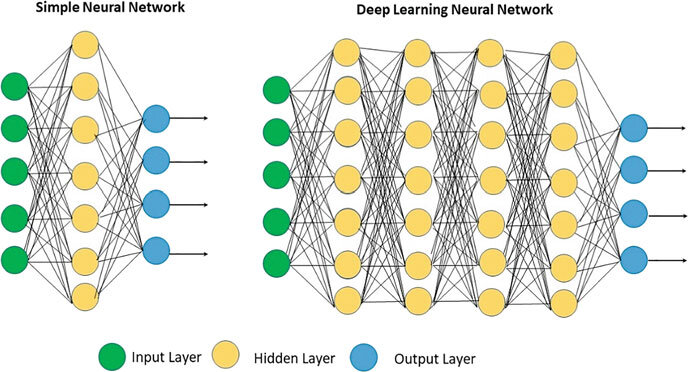
\includegraphics[width=0.8\textwidth]{imgs/neural_vs_deep.png}
\caption{Comparison between traditional neural networks (left) and deep learning architectures (right), illustrating the difference in complexity and hierarchical feature learning capabilities.}
\label{fig:neural_vs_deep}
\end{figure}

Deep learning architectures consist of multiple hidden layers, each containing many artificial neurons (nodes) that process information through weighted connections. Each neuron receives inputs, applies a weighted sum followed by an activation function, and passes the result to subsequent layers. This layered structure enables the network to learn increasingly complex and abstract representations, with early layers capturing low-level features and deeper layers combining these into high-level patterns. The depth of these networks allows them to model complex, non-linear relationships that are particularly valuable for complex temporal data such as battery wear patterns.

For this project, the deep learning approach was specifically chosen due to its superior ability to capture complex temporal patterns inherent in battery wear data and its capacity to handle the high-dimensional, sequential nature of battery health monitoring without requiring extensive domain-specific preprocessing or manual feature design. Deep learning excels in battery applications because it can automatically discover relevant features from raw sensor measurements (voltage, current, temperature) and learn the subtle, non-linear relationships between these measurements and battery health states~\cite{noauthor_comprehensive_nodate}. The hierarchical feature learning capability is particularly important for battery data, where wear patterns show across multiple time scales and involve complex interactions between chemical processes. Furthermore, deep learning architectures such as RNNs, LSTM networks, and Transformers are specifically designed to handle sequential data, making them ideal for modeling the temporal dependencies present in battery operational data and predicting future health states based on historical patterns. as this paper demonstrates, Transformer-based approaches are effective for battery RUL prediction~\cite{chen_transformer_2022}.


Understanding key training parameters and concepts is crucial for developing effective battery state estimation models. The most relevant of these are:

\begin{itemize}
    \item \textbf{Epochs} represent complete passes through the training dataset, where 50--500 epochs are typical for battery data, carefully balancing the risk of underfitting with too few iterations against overfitting with excessive training on temporal sequences.
    \item \textbf{Batch Size} determines the number of samples processed at the same time, where smaller batches (16--32) excel at capturing nonlinear patterns in battery behavior, while larger batches (128--256) provide more stable gradients but may struggle with the irregular nature of real-world battery data.
    \item \textbf{Patience} in early stopping mechanisms defines how many epochs to wait without validation improvement before ending training, with values of 5--20 epochs proving effective at preventing overfitting while allowing models sufficient time to generalize across different battery systems and operational conditions.
    \item \textbf{Learning Rate} controls the size of parameter adjustments during training, requiring careful tuning for battery wear patterns: rates too high (>0.01) risk missing subtle wear signals, while rates too low (<0.0001) result in painfully slow convergence and potentially incomplete learning.
    \item \textbf{Optimizers} play a critical role in training efficiency, with the Adam optimizer commonly chosen for its adaptive learning rate capabilities, while SGD with momentum provides more stable convergence but demands additional hyperparameter tuning specifically for battery applications.
    \item \textbf{Regularization} techniques, including L1/L2 regularization and dropout, become particularly important when working with limited battery datasets, especially when training data comes from only a few battery types or specific operational conditions.
     \item \textbf{Loss Functions} must be carefully selected based on the specific task: MSE for regression problems like SoC and capacity prediction, MAE when robustness against outliers is most important, cross-entropy for classification tasks such as fault detection, and custom loss functions that can elegantly incorporate domain-specific knowledge about battery behavior. Finally,
    \item \textbf{Validation} strategies require special consideration in battery applications, where time-based splitting ensures models are tested on genuinely future data, and cross-validation procedures must account for the inherent temporal dependencies present in battery wear sequences.
\end{itemize}


\subsection{Battery Degradation and Aging}
\label{sec:degradation}

Battery wear refers to the gradual loss of a battery's ability to store and deliver energy, driven by chemical reactions, temperature changes, charge/discharge cycles, and aging. This wear shows as capacity fade, resulting in reduced device runtime or diminished electric vehicle driving range. Figure~\ref{fig:degradation_mechanisms} illustrates the various degradation mechanisms that occur within lithium-ion battery cells during operation and aging.

\begin{figure}[htbp]
\centering
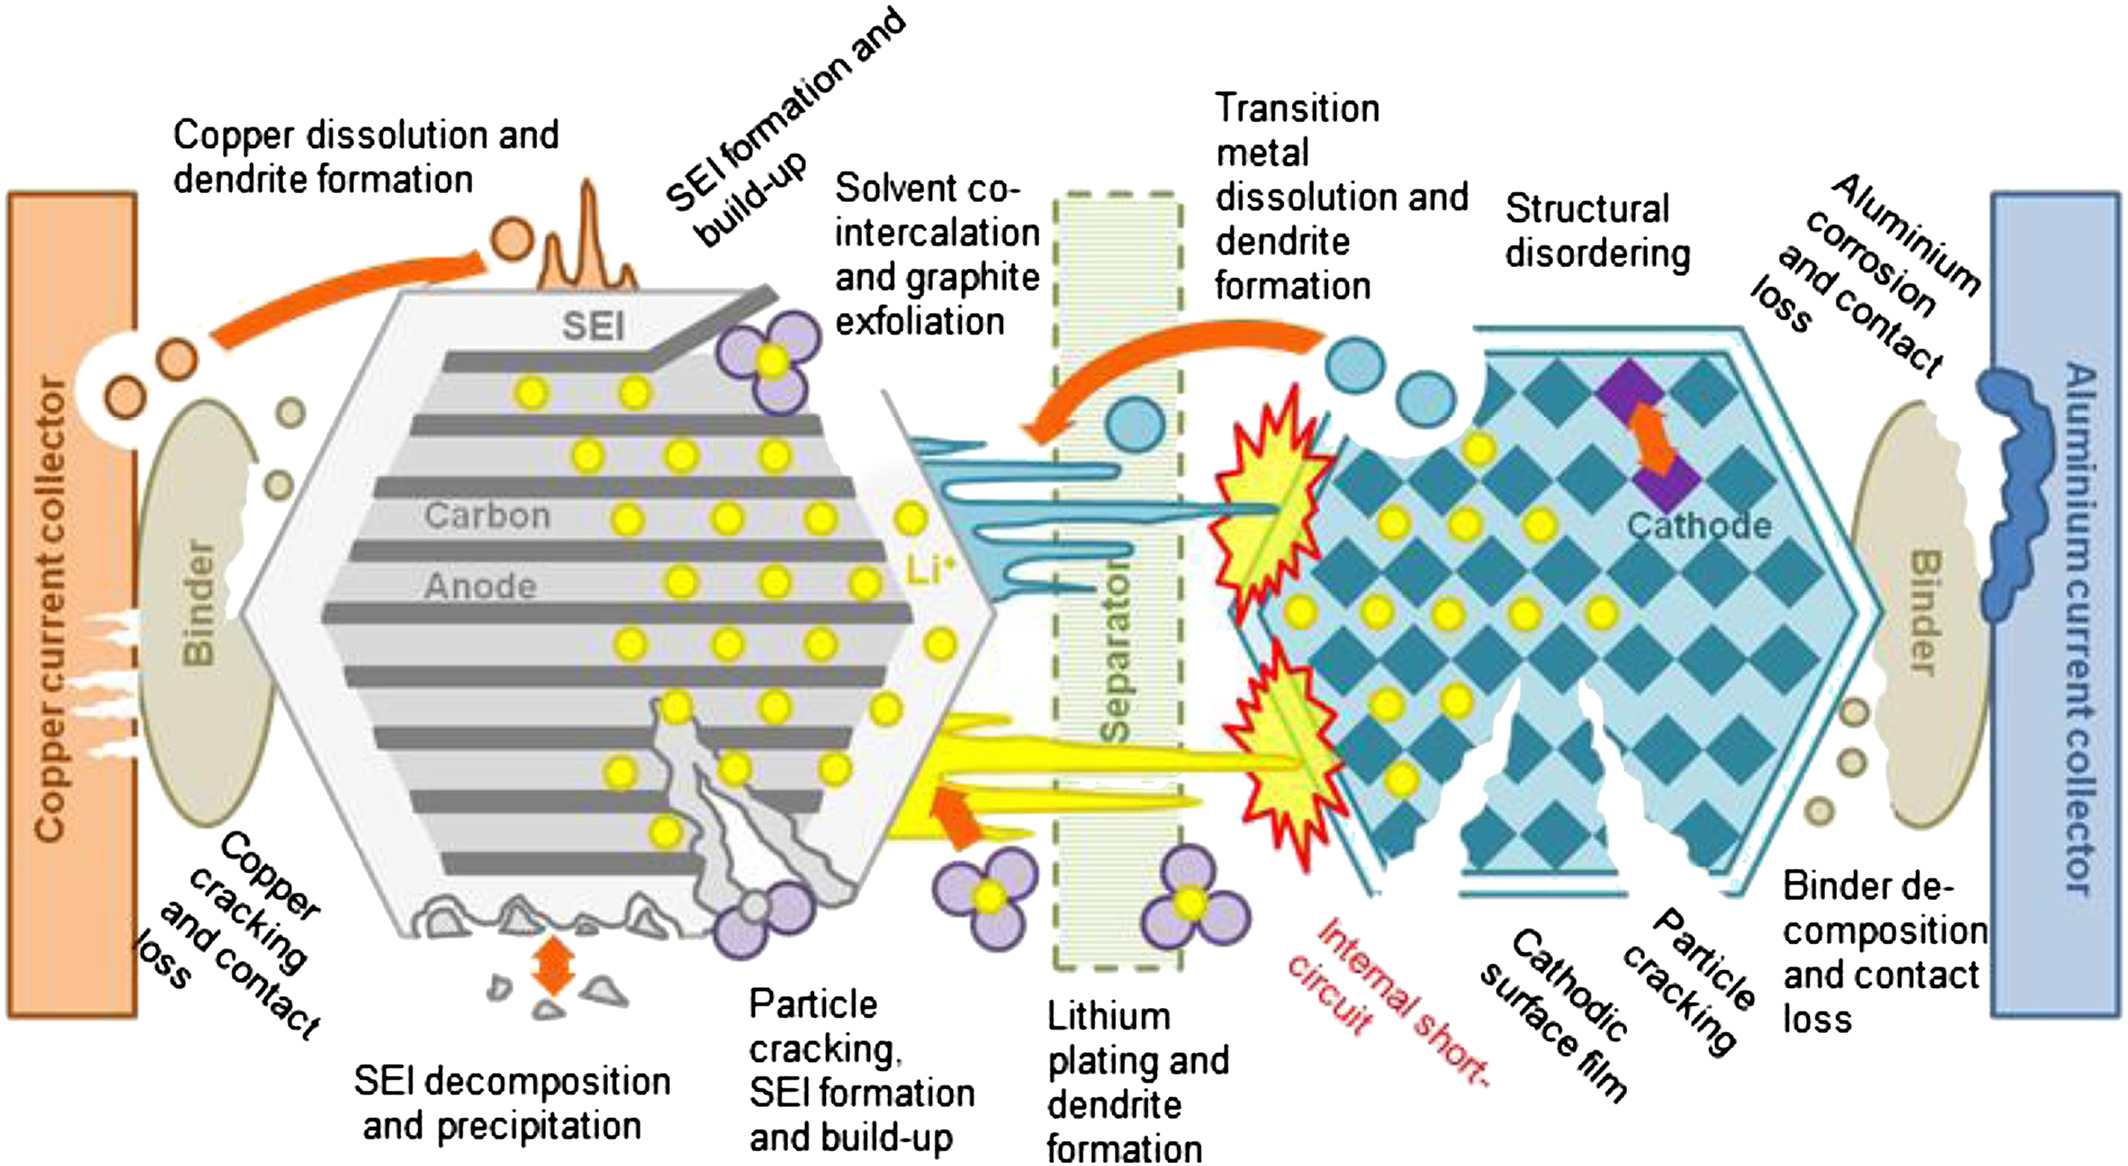
\includegraphics[width=0.9\textwidth]{imgs/Degradation mechanisms in Li-ion cells.jpg}
\caption{Degradation mechanisms in lithium-ion battery cells, showing various chemical and physical processes that contribute to battery wear and capacity loss over time. From \cite{kabir_degradation_2017}.}
\label{fig:degradation_mechanisms}
\end{figure}

The key mechanisms contributing to this wear include several interconnected processes. \textbf{SEI Growth} occurs when a layer forms on the anode, consuming lithium ions and reducing capacity. This process is accelerated at high temperatures and currents, leading to an initial irreversible capacity loss of approximately 10\% during formation cycles. \textbf{Lithium Plating} represents another critical mechanism where, at low temperatures or high charge rates, lithium deposits on the anode, forming ``dead lithium'' that contributes to irreversible capacity loss and increases safety risks. \textbf{Particle Fracture} results from mechanical stress during cycling, causing cracks in electrode materials that reduce active material availability and make capacity decline worse. \textbf{PE Decomposition} involves structural changes in the cathode, such as spinel/rock salt phase formation, which degrade performance and contribute to active material loss. Finally, \textbf{Impedance Increase} shows as rising interfacial resistance, mainly at the positive electrode, which limits efficient charge transfer and indirectly reduces usable capacity. After 800 cycles, electrode resistance can increase tenfold, significantly impacting battery performance. The authors in \cite{zhang_studies_2000} discuss the \textbf{Capacity Fade} mechanism, that refers to the progressive decline in the ability of a lithium-ion battery to store energy, manifested as a reduced device runtime or a reduced electric vehicle driving range. Capacity losses range from 12.4\% to 32\% after 500--800 cycles, corresponding to an average loss of 0.025--0.05\% per cycle.

As lithium ion batteries age, their internal resistance increases, badly affecting power delivery, charging efficiency, and thermal management. This wear is particularly noticeable during calendar aging, as detailed in the study by \cite{stroe_degradation_2018} on LFP/C-based batteries. The primary mechanisms contributing to this increase involve several interconnected processes. \textbf{SEI Growth} is characterized by the thickening of the SEI layer on the graphite anode over time, reducing Li$^+$ ion permeability. This growth follows a power law dependence (approximately $t^{0.8}$) and is accelerated at high temperatures and high SOC levels, leading to increased resistance and contact loss within the anode. \textbf{Lithium Plating} involves the deposition of metallic lithium on the anode, which clogs electrode pores, blocking ion transport and elevating resistance, particularly under high SOC conditions. \textbf{Cathode Structural Degradation} occurs at the LFP cathode, where binder decomposition, oxidation of conductive agents, and corrosion of current collectors reduce inter-particle conductivity, contributing to resistance increase, especially at elevated temperatures. Also, \textbf{Electrolyte Decomposition} produces decomposition products that form resistive surface layers on both electrodes, further increasing internal resistance, with effects amplified at high temperatures and SOC levels. This same study shows that internal resistance increases nonlinearly with storage time, with exponential acceleration due to higher storage temperatures (e.g., 55°C) and SOC levels (e.g., 90\%). For instance, after 20 years at 25°C and 50\% SOC, resistance may rise by approximately 71\%, doubling at 100\% SOC. This increased resistance results in slower charging, reduced power output, and accelerated wear due to enhanced heat generation, impacting battery performance and lifespan.

For these reasons, battery health monitoring is critical for ensuring reliability, safety, and longevity of battery systems. Monitoring involves checking key parameters such as SoC and SoH, which provide essential insights into battery performance and remaining operational capacity. However, this is not and easy task and many challenges must be overcome. 



\subsection{Challenges of Battery Health Monitoring}
The technical challenges in monitoring battery health come from the complex nature of battery systems and the difficulties in accurately estimating SOC and SOH.

\begin{itemize}
    \item \textbf{Complexity of Battery Chemistry}: Batteries, particularly lithium-ion batteries, have complex internal chemistry that are difficult to model and monitor.
    \item Factors such as temperature, charge-discharge rates, and depth of discharge influence wear, making accurate SOH estimation challenging. Also, the nonlinear and complex wear processes vary with usage conditions, environmental factors, and battery design, complicating predictive modeling.
    \item \textbf{Measurement Difficulties}: Measuring individual battery parameters, such as internal resistance, temperature, and voltage, is technically challenging, especially in real-time applications.  This requires precise sensors and sophisticated equipment, which may not be possible in real-world scenarios.
    \item For instance, accurately measuring internal resistance or temperature in a moving vehicle is far more complex than in a controlled lab environment.
    \item \textbf{Modeling and Estimation}: Developing accurate models for SOH estimation is complex. Chemical models, which simulate battery behavior based on physical and chemical principles, require extensive computational resources and detailed parameter inputs (e.g., electrolyte properties, reaction rates). Semi-empirical models often oversimplify chemical processes, reducing their effectiveness under extreme conditions. Equivalent circuit models (ECMs) may lack precision during high-rate charging/discharging or extreme temperatures due to their simplified nature.
    \item \textbf{Limitations of Data-Driven Methods}: Data-driven approaches, such as machine learning techniques (e.g. Support Vector Regression, Gaussian Process Regression, Artificial Neural Networks), rely on large, high-quality datasets, which can be difficult to obtain. These methods also lack physical understanding, making it difficult to understand their predictions. Also, issues like overfitting and high computational demands pose challenges for real-time applications.
    \item \textbf{Complexity of Hybrid Methods}: Hybrid approaches, which combine model-based and data-driven methods, can improve accuracy but increase system complexity and computational costs. Understanding errors in these systems remains a challenge, requiring further research to enhance transparency and efficiency.
    \item \textbf{Laboratory vs Real World Conditions}: There is a significant difference between laboratory-simulated conditions and actual operational environments. Laboratory settings often use sophisticated equipment that is not available in real-world applications, limiting the applicability of monitoring methods. For example, real-world conditions like varying temperatures or road vibrations are difficult to replicate in a lab, affecting SOH estimation accuracy.
    \item \textbf{Real-Time Monitoring}: Getting real-time, reliable SOH monitoring is crucial for safety-critical applications but is technically demanding. BMS must balance accuracy with computational efficiency to provide timely insights without overloading system resources.
    \item \textbf{Environmental Factors}: Batteries are sensitive to environmental conditions such as temperature, humidity, and vibration. Monitoring systems must account for these factors, which can significantly impact battery health and performance.
    \item For example, high temperatures can accelerate battery wear, while low temperatures may reduce capacity, complicating health estimation.
    \item \textbf{Cost of Monitoring Systems}: Setting up sophisticated battery health monitoring systems can be expensive, both in terms of initial setup and ongoing maintenance. This includes the cost of sensors, data storage, and computational infrastructure, which can be too expensive for smaller organizations or applications.
    \item \textbf{Data and Computational Costs}: AI and data-driven methods require significant computational resources and high-quality data, which can be costly to acquire and process. The high demand for data and computing power presents challenges, particularly for real-time monitoring applications and edge devices.
\end{itemize}

%\section{Supporting Technologies}
%Sensor technologies for battery data collection
%Data acquisition systems and protocols
%Computing platforms/hardware used

%\section{Methodogical Background}
%Signal processing techniques for battery data
%Feature extraction methods
%Relevant machine learning algorithms (classification, regression, etc.)
%Evaluation metrics for health monitoring systems

%\section{Related Frameworks}
%Software libraries and tools used in implementation
%Data management approaches
%Visualization techniques

\section{Supporting Technologies}

This section describes the complete suite of software tools and platforms that helped the research and development process, including analytical frameworks, optimization tools, and development environments.

\subsection{Data Analysis Tools}


\textbf{Weights and Biases (WandB)}
\label{subsec:wandb}
WandB is a machine learning platform designed for experiment tracking and display~\cite{noauthor_weights_nodate}. It enables real-time logging and monitoring of training metrics, parameters, and model outputs. In this study, WandB was used to keep track of training processes and display losses, providing interactive dashboards to analyze experiments.

\textbf{PlotJuggler}
PlotJuggler is an open-source time series display tool designed for fast, easy-to-use, and extensible data analysis~\cite{faconti_facontidavideplotjuggler_2025}. It features a user-friendly drag-and-drop interface, enabling efficient display of large datasets. In this work, PlotJuggler was highly effective for exploring and analyzing data within datasets, allowing for the display of time series, identification of patterns. Its a valuable tool for detailed data inspection and analysis.

\textbf{Orange Data Mining}
Orange Data Mining is an open-source data display and analysis platform designed for exploratory data analysis and machine learning workflows~\cite{noauthor_biolaborange3_nodate}. It provides a visual programming interface with drag-and-drop widgets that enable users to build data analysis pipelines without extensive coding. Orange offers complete tools for data preprocessing, feature selection, correlation analysis, and outlier detection through interactive displays and statistical methods. In this work, Orange was important for exploring correlations within battery datasets and identifying outliers that could potentially skew model performance.

\subsection{Development Tools and Frameworks}



\textbf{Git Version Control}
Git is a distributed version control system designed to handle projects of all sizes with speed and efficiency~\cite{noauthor_git_nodate}. It tracks changes in source code and files during software development,maintaining a complete history of modifications. Git provides features such as branching, merging. In this work, Git was used to ensure version control throughout the research process, maintaining a complete history of code changes, experimental iterations, and documentation updates. All project files, including machine learning models, data processing scripts, and analysis, were committed and pushed to GitHub repositories.

\textbf{Conda Environments}
Conda is an open-source package management and environment management system that simplifies the installation, running, and updating of packages and 
their dependencies~\cite{conda_contributors_conda_2025}. It creates isolated environments where different versions of Python, libraries, 
and dependencies can coexist without conflicts, making it particularly valuable for this projects. This approach ensured that version conflicts between packages were avoided, enabled smooth collaboration across different 
development machines, and guaranteed that the exact software environment could be recreated for reproducibility.

\textbf{Optuna}
\label{subsec:optuna}
Optuna is an open-source hyparameter tuning framework used to search for the best parameters in machine learning models~\cite{akiba_optuna_2019}. It uses algorithms like TPE to systematically explore parameter spaces, supporting parallel and distributed optimization. In this work, Optuna was used to automate the tuning process, improving model performance by identifying optimal parameter configurations with reduced manual effort.

\textbf{PyTorch}
PyTorch is an open-source machine learning framework developed by Facebook's AI Research lab, designed for deep learning applications with a 
focus on flexibility and ease of use~\cite{ansel_pytorch_2024}. It provides dynamic computational graphs, 
allowing for easy model development and debugging through its eager execution model. PyTorch features 
automatic differentiation capabilities through its autograd system, enabling efficient gradient computation 
for backpropagation in neural networks. The framework supports GPU acceleration through CUDA, making it suitable
for training large-scale models efficiently. 

PyTorch was specifically chosen over TensorFlow for this project due to several key advantages that align with the research requirements. \textbf{Research-oriented design} provides greater flexibility for implementing novel architectures and custom loss functions specific to battery wear modeling, whereas TensorFlow's static graph approach can be more restrictive for experimental work. Also, \textbf{superior community support} in the academic research community and \textbf{extensive documentation}.

In this work, PyTorch served as the primary framework for developing and training deep learning models for battery health monitoring applications. PyTorch smoothly integrates with other tools in the machine learning pipeline, such as Optuna (see Section~\ref{subsec:optuna}) for automated parameter tuning and WandB (see Section~\ref{subsec:wandb}) for comprehensive experiment tracking, creating a cohesive development environment that supports reproducible research workflows.




\cleardoublepage%************************************************
\chapter{State of the Art}
\label{ch:stateoftheart}
%************************************************
\color{Red}comentário geral. Podia densificar um pouco mais e acrescentar figuras/tabelas (mesmo que sejam dos artigos que refere). Basta colocar a referencia na legenda. Ficava bem uma figura com a taxonomia  dos metodos\color{Black}

Getting the right predictions for SoC, SoH, and RUL is very important for making batteries work better in cars and trains. These predictions help make battery management systems (BMS) more reliable and work better. They provide key information for watching battery health and planning when to fix or replace batteries. Traditional methods, like Coulomb Counting and Kalman Filters, often have trouble with complex battery behavior and changing conditions. New advances in Artificial Intelligence (AI), especially machine learning and deep learning, provide better solutions by finding complex patterns in battery data. This chapter looks at the current best methods for SoC, SoH, and RUL estimation, focusing on AI-based approaches.

\section{Battery State Estimation}

\subsection{Traditional Methods}
\label{subsec:traditional_methods}
Traditional methods for checking battery state can be put into two groups: physics-based and statistical approaches, each with built-in problems.

\textbf{Physics-Based Methods} create models of how batteries work chemically and electrically. Key approaches include:
\begin{itemize}
    \item \textbf{Equivalent Circuit Models (ECMs)}: Show batteries using electrical parts (like resistors, capacitors) to copy voltage and current behavior. ECMs represent battery dynamics through simplified electrical circuits that capture the essential electrochemical behaviors while maintaining computational efficiency. Figure~\ref{fig:ecm_models} illustrates two common ECM configurations: (a) the Thévenin model with a single RC pair representing charge transfer resistance and double-layer capacitance, and (b) the Partnership for a New Generation of Vehicles (PNGV) model with multiple RC pairs capturing different time constants in battery response. These models include internal resistance ($R_0$), polarization resistances ($R_{Th}$, $R_{pa}$, $R_{pc}$), and corresponding capacitances ($C_{Th}$, $C_{pa}$, $C_{pc}$) to model various electrochemical processes. ECMs are fast to compute and suitable for real-time applications, but they are not very accurate when conditions change and require parameter identification for different operating conditions \cite{tran_comparative_2021}.

\begin{figure}[htbp]
\centering
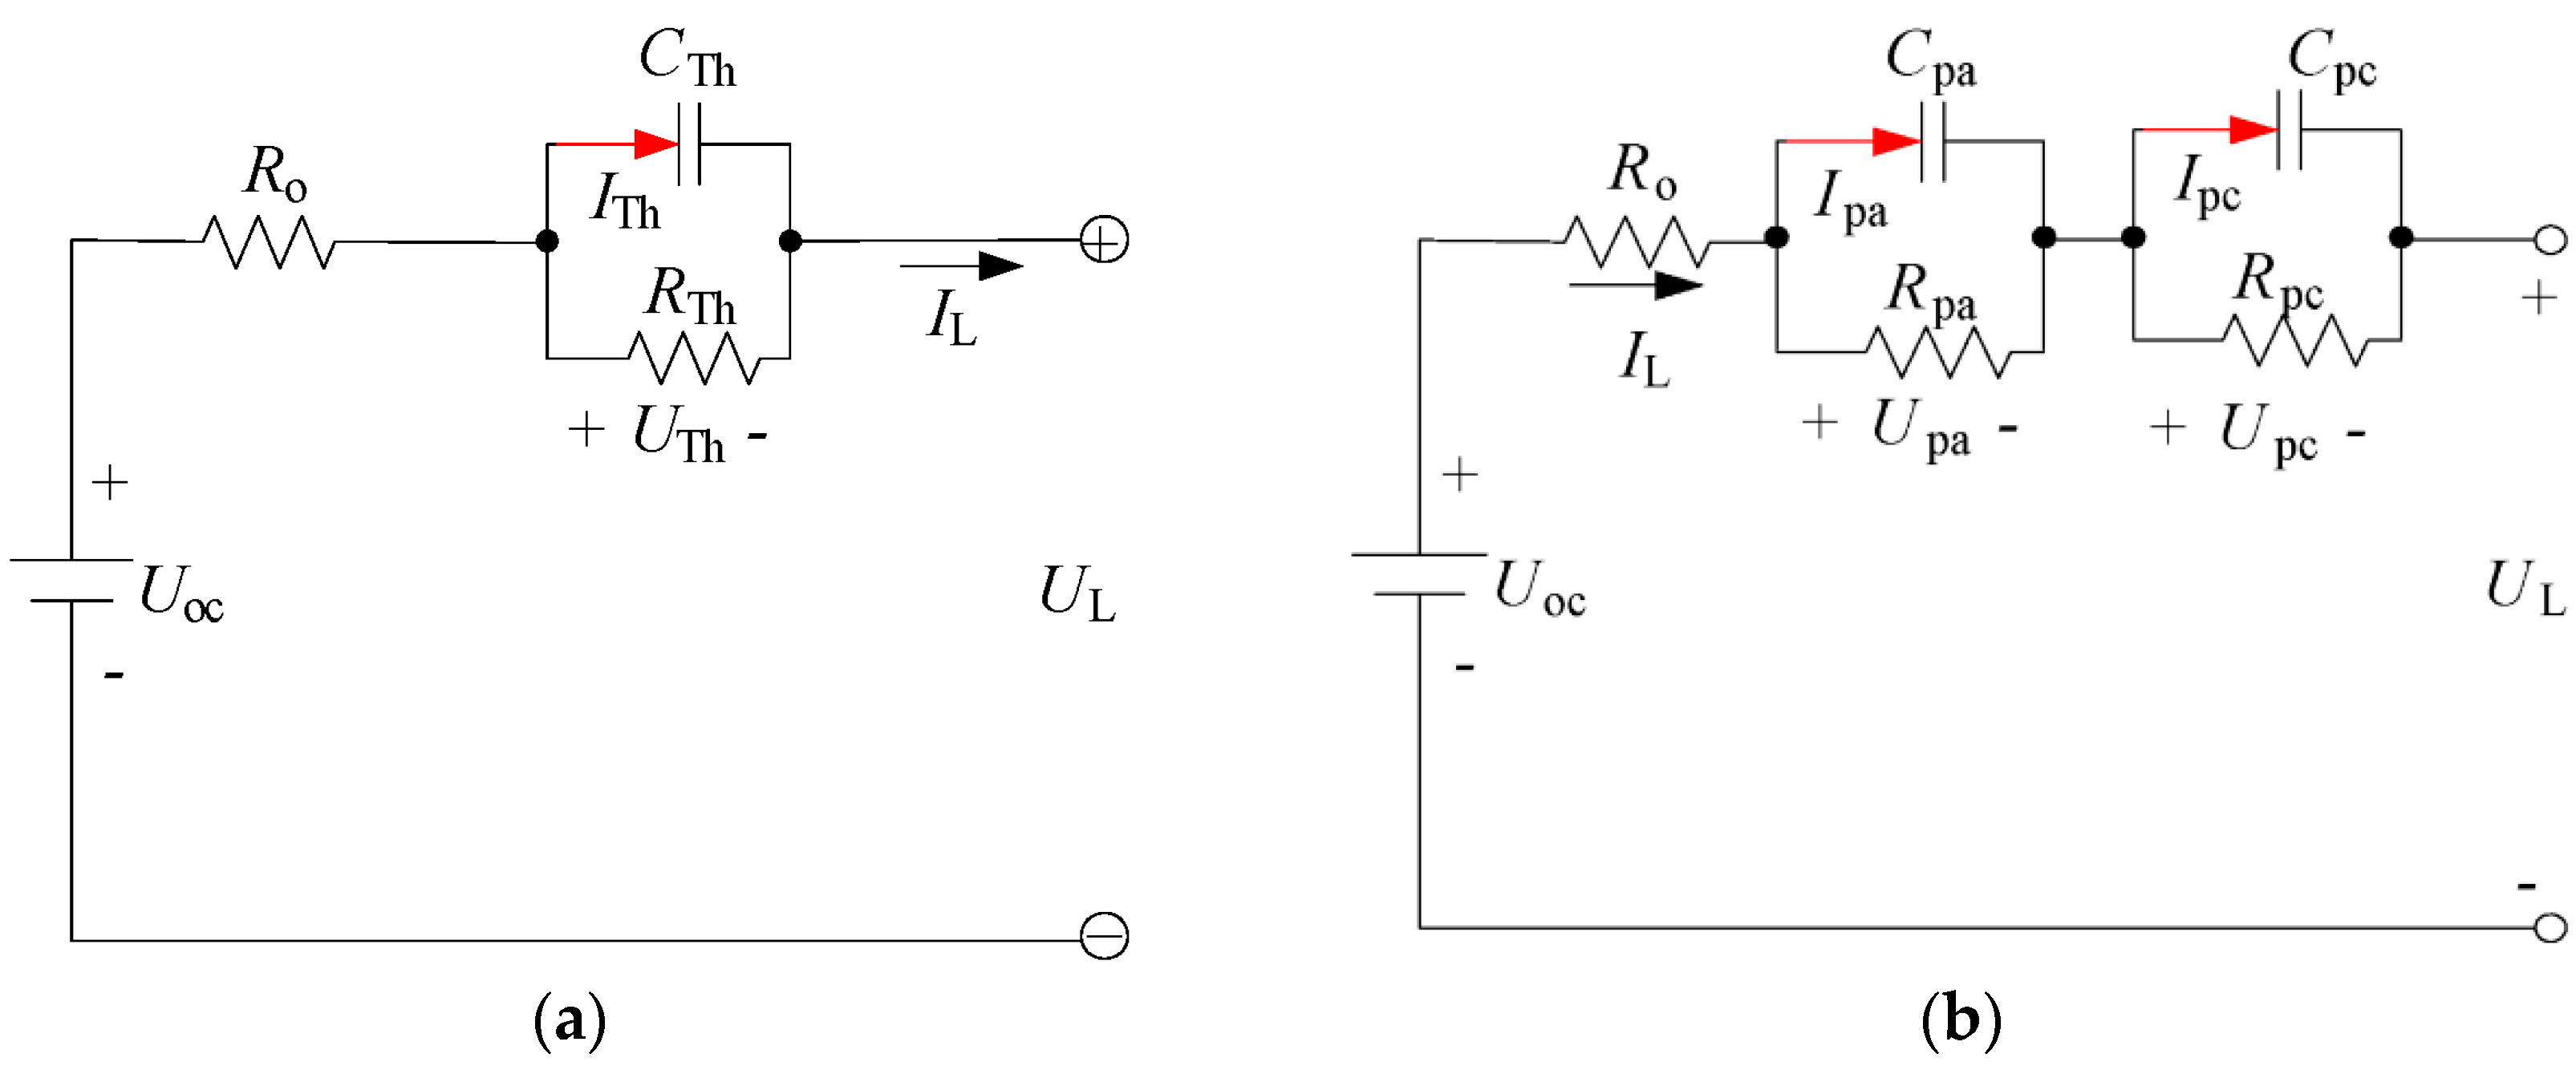
\includegraphics[width=1.0\textwidth]{imgs/ECM_1st_2nd_order.png}
\caption{Equivalent Circuit Models (ECMs) showing (a) Thévenin model with single RC pair and (b) PNGV model with multiple RC pairs. These models use electrical components to represent battery electrochemical behavior, where $R_0$ represents ohmic resistance, $R_{Th}/C_{Th}$ and $R_{pa}/C_{pa}$, $R_{pc}/C_{pc}$ represent different polarization effects with their respective time constants \cite{tran_comparative_2021}.}
\label{fig:ecm_models}
\end{figure}

    \item \textbf{Electrochemical Models}: Copy internal chemical reactions, giving high accuracy but needing a lot of computer power and detailed knowledge of battery parameters. These models are based on fundamental electrochemical principles and describe the physical and chemical processes occurring within battery cells, including ion transport, charge transfer reactions, and material phase changes \cite{mama_comprehensive_2025}. Electrochemical models typically solve complex partial differential equations that describe mass and charge conservation, making them computationally intensive but highly accurate for predicting battery behavior under various operating conditions.

    A notable example of modern electrochemical modeling frameworks is BattMo (Battery Modeling in MATLAB), an open-source battery simulation platform that provides comprehensive tools for electrochemical battery modeling \cite{noauthor_battmo_2024}. BattMo offers advanced capabilities including multi-physics coupling, detailed electrode modeling, and thermal effects integration, making it suitable for research and development applications.

    During the initial phases of this research, BattMo was evaluated as a potential modeling framework for generating synthetic battery data and understanding fundamental battery behavior. The platform's comprehensive approach to electrochemical modeling and its integration with MATLAB made it an attractive option for physics-based battery simulation. However, after preliminary exploration, the focus shifted toward data-driven approaches due to the computational complexity requirements and the need for extensive parameter identification that electrochemical models demand for practical applications in real-time battery management systems.
\end{itemize}

Unlike these, \textbf{ statistical methods} use real data to estimate battery states. Common methods include:
\begin{itemize}
    \item \textbf{Coulomb Counting}: This method estimates SoC by integrating current over time, following the fundamental principle that charge accumulation equals the integral of current. While conceptually straightforward, coulomb counting suffers from significant practical limitations including sensitivity to measurement noise, current sensor drift, and initialization errors. Figure~\ref{fig:current_integration_error} illustrates how current integration errors accumulate over time, demonstrating the inherent challenges of this approach. The method's accuracy degrades particularly under varying sampling rates and temperature conditions~\cite{noauthor_implementation_nodate}. Despite these limitations, coulomb counting remains widely used due to its computational simplicity, often serving as a baseline method or being combined with other estimation techniques for improved reliability~\cite{movassagh_critical_2021}.

\begin{figure}[htbp]
\centering
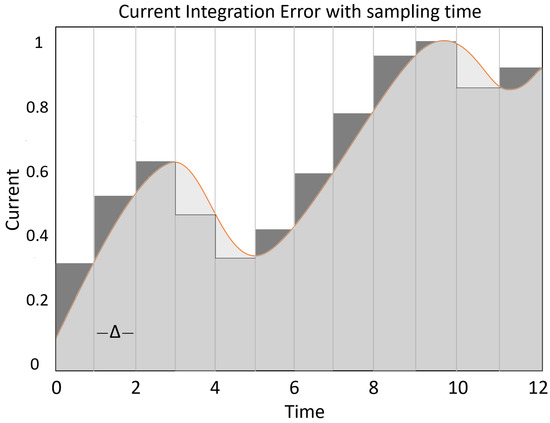
\includegraphics[width=0.8\textwidth]{imgs/coulomb.jpg}
\caption{Current integration error accumulation over time showing how measurement uncertainties and sampling effects impact coulomb counting accuracy. The step-like behavior demonstrates the discrete nature of current sampling, while the smooth curve represents the theoretical continuous integration~\cite{movassagh_critical_2021}.}
\label{fig:current_integration_error}
\end{figure}

    \item \textbf{Kalman Filters}: Kalman filters represent a sophisticated recursive approach to state estimation that optimally combines model predictions with noisy measurements using statistical principles. The filter operates in two phases: prediction (using system dynamics) and correction (incorporating new measurements). For battery applications, the Extended Kalman Filter (EKF) is commonly employed to handle the nonlinear relationship between battery states and observable quantities such as terminal voltage~\cite{mastali_battery_2013}. Figure~\ref{fig:ekf_diagram} illustrates the EKF estimation process, showing how the algorithm iteratively refines state estimates by balancing model predictions with measurement data. While Kalman filters provide optimal estimates under Gaussian noise assumptions, their performance degrades significantly when dealing with the complex nonlinear dynamics and time-varying parameters characteristic of battery systems. The method requires accurate system models and proper tuning of noise covariance matrices, which can be challenging in practical applications where battery parameters drift over time due to aging and temperature variations~\cite{becker_wwwkalmanfilternet_online_nodate}.

\begin{figure}[htbp]
\centering
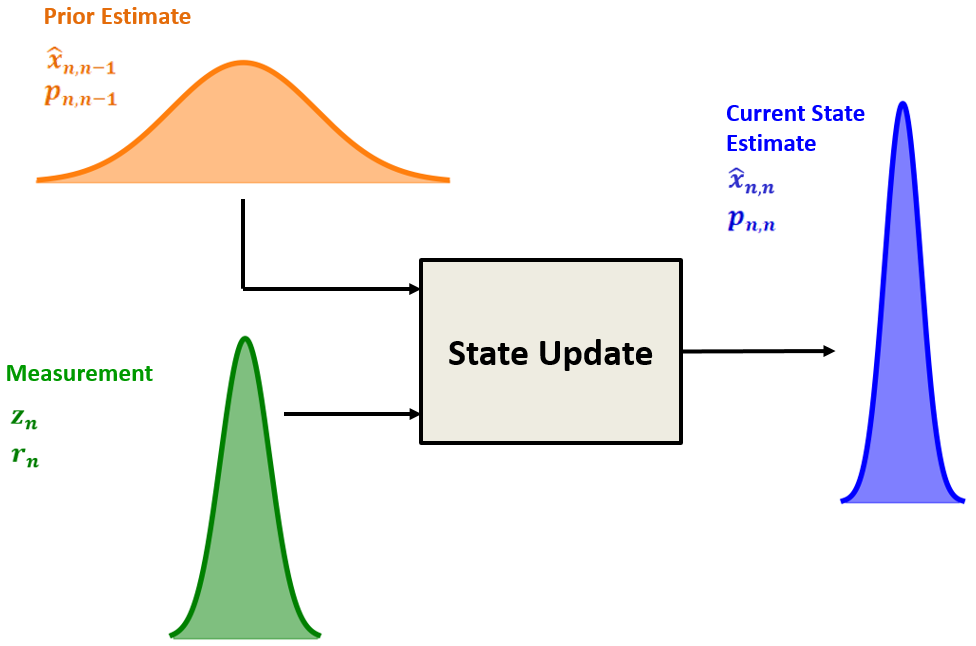
\includegraphics[width=0.9\textwidth]{imgs/ekf.png}
\caption{Extended Kalman Filter (EKF) State estimation process showing Prior Estimate (orange), Measurement (green), State Update (gray), and Current State Estimate (blue).~\cite{becker_wwwkalmanfilternet_online_nodate}.}
\label{fig:ekf_diagram}
\end{figure}
    
\end{itemize}

Because these methods often fail to capture small changes in battery behavior when conditions change, multiple AI-based approaches have been proposed in the last decade.

\subsection{AI-Based Methods}
\label{subsec:ai_methods}
AI-based methods use machine learning and deep learning to model complex relationships in battery data. This section looks at key approaches, datasets, and how they're used in this project.

\textbf{Machine Learning} algorithms that learn from examples, such as Support Vector Machines (SVMs) and Random Forests, have been used to predict SoC and SoH using features like voltage, current, and temperature. For example, \cite{sun_simultaneous_2022} shows SVMs getting high accuracy in SoH estimation (98.26\%) for lead-acid batteries under controlled conditions. However, these methods need a lot of feature engineering and have trouble with time-based patterns. On the contrary, \textbf{Deep Learning} models are very good at finding time-based and spatial patterns in battery data. Key types include:
\begin{itemize}
    \item \textbf{Convolutional Neural Networks (CNNs)}: Find spatial features from battery data, such as voltage profiles. Combining CNNs with Long Short-Term Memory (LSTM) units, as done in the \cite{Fangfang_Yang} paper, makes forecasting more accurate by modeling time-based patterns.
    \item \textbf{Recurrent Neural Networks (RNNs) and LSTMs}: Made for sequential data, LSTMs are very good for RUL prediction, as they capture long-term battery wear trends. The key advantage of LSTMs over traditional RNNs lies in their ability to selectively remember and forget information through specialized gate mechanisms, as illustrated in Figure~\ref{fig:rnn_vs_lstm_comparison}. While standard RNNs suffer from vanishing gradient problems that limit their ability to capture long-term dependencies, LSTMs incorporate long-term memory cells alongside working memory, enabling effective modeling of extended battery degradation sequences. This architectural improvement is crucial for battery applications where degradation patterns span hundreds or thousands of cycles \cite{noauthor_phenomnet_nodate}. Studies using the NASA Battery Dataset \cite{noauthor_nasa_nodate} show LSTM-based models work better than older methods in RUL estimation as done in the \cite{hong_state--health_2023}.

\begin{figure}[htbp]
\centering
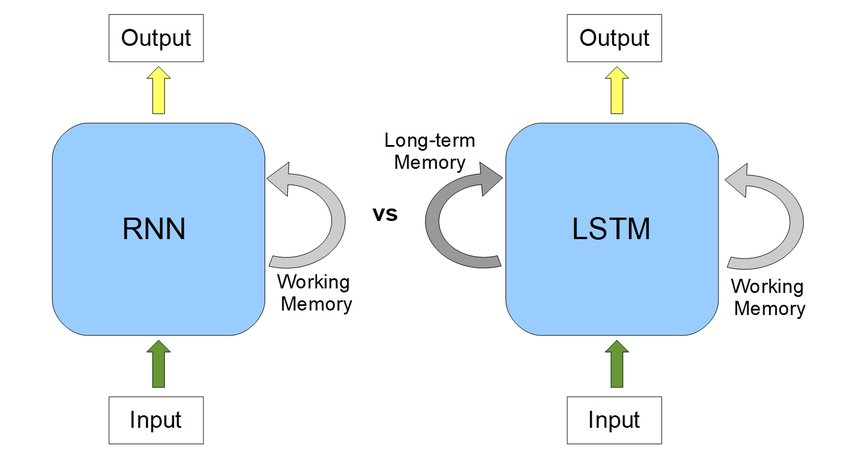
\includegraphics[width=1\textwidth]{imgs/rnn_lstm.png}
\caption{Comparison between RNN and LSTM architectures showing the fundamental difference in memory mechanisms. RNNs rely solely on working memory with limited long-term retention capabilities, while LSTMs incorporate both working memory and long-term memory cells, enabling better modeling of extended temporal dependencies in battery degradation data \cite{noauthor_phenomnet_nodate}.}
\label{fig:rnn_vs_lstm_comparison}
\end{figure}

    \item \textbf{Transformer Models}: New in battery state estimation, transformers use attention mechanisms to model complex dependencies, showing promise in handling different-length sequences \cite{yilmaz_transformer-based_2025}. The Transformer architecture, illustrated in Figure~\ref{fig:transformer_detailed_architecture}, consists of an encoder-decoder structure with multiple specialized components. The encoder processes input sequences through multiple layers containing self-attention mechanisms, positional encoding, and feed-forward networks, enabling the model to capture long-range dependencies in battery time series data. The decoder utilizes both self-attention and encoder-decoder attention mechanisms to generate predictions, with linear mapping layers producing the final output. This architecture is particularly effective for battery applications because the attention mechanisms can automatically identify relevant temporal patterns and relationships between different time steps in battery degradation sequences, eliminating the need for manual feature engineering while maintaining computational efficiency through parallel processing capabilities.
\end{itemize}

\begin{figure}[htbp]
\centering
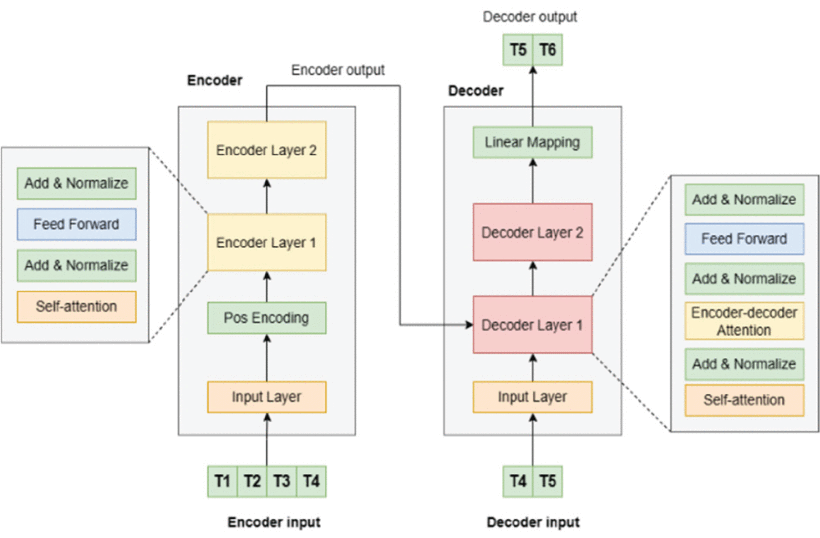
\includegraphics[width=0.9\textwidth]{imgs/transformer_input.png}
\caption{Detailed Transformer architecture showing the encoder-decoder structure with self-attention mechanisms, positional encoding, and feed-forward networks. The encoder processes input sequences (T1-T4) while the decoder generates output predictions (T5-T6) using attention mechanisms to capture temporal dependencies in battery data.}
\label{fig:transformer_detailed_architecture}
\end{figure}

\subsection{Hybrid Approaches}
\color{Red}faltam referências nesta subsecção\color{Black}
Hybrid models combine physics-based and data-driven methods to make results more accurate. For example, some studies combine ECMs with neural networks to improve SoC estimates, using physical constraints to reduce the amount of training data needed. Such approaches are very useful for railway applications, where operating conditions change a lot. Despite improvements, several challenges still exist in battery state estimation:
\begin{itemize}
    \item \textbf{Data Requirements}: AI models, especially deep learning, need large, varied datasets, which are often limited or private.
    \item \textbf{Operating Variability}: Battery performance changes due to temperature, load profiles, and aging, making it hard for models to work in different situations.
    \item \textbf{Computer Complexity}: Real-time estimation in cars and trains needs fast models, which is a challenge for complex deep learning systems.
    \item \textbf{Lack of Standard Datasets}: The absence of universal, open-source datasets for railway applications limits model comparison and testing.
\end{itemize}


\section{Datasets for AI-Based Estimation}
\label{subsec:datasets}
The quality and variety of datasets are very important for training strong AI models. A comprehensive analysis of available battery datasets reveals significant variation in data completeness, experimental conditions, and feature availability. Table~\ref{tab:battery_datasets_comparison} presents a detailed comparison of notable publicly available battery datasets, highlighting their characteristics and available measurements.

\begin{table}[htbp]
\centering
\caption{Comprehensive comparison of available battery datasets and their features}
\label{tab:battery_datasets_comparison}
\resizebox{\textwidth}{!}{%
\begin{tabular}{lcccccccccccccccc}
\hline
\textbf{Dataset} & \textbf{Cell Type} & \textbf{Chemistry} & \textbf{Time} & \textbf{C/D Ind.} & \textbf{Cycle} & \textbf{Current} & \textbf{Voltage} & \textbf{Dis. Cap.} & \textbf{Ch. Cap.} & \textbf{Ch. Energy} & \textbf{Dis. Energy} & \textbf{dV/dt} & \textbf{Int. Res.} & \textbf{AC Imp.} & \textbf{ACI Phase} & \textbf{Temp.} \\
\hline
Zn-ion, Na-ion @2025 & Various & Zn-ion, Na-ion & $\checkmark$ & $\checkmark$ & & $\checkmark$ & $\checkmark$ & $\checkmark$ & $\checkmark$ & & & & & & & \\
CALCE CS2 @2010 & Prismatic & LiCoO2 & $\checkmark$ & $\checkmark$ & $\checkmark$ & $\checkmark$ & $\checkmark$ & $\checkmark$ & $\checkmark$ & $\checkmark$ & $\checkmark$ & $\checkmark$ & $\checkmark$ & $\pm$ & $\pm$ & Initial \\
MATR @2019 & 18650 & LFP/graphite & $\checkmark$ & $\checkmark$ & $\checkmark$ & $\checkmark$ & $\checkmark$ & $\checkmark$ & $\checkmark$ & $\checkmark$ & $\checkmark$ & $\checkmark$ & $\checkmark$ & & & $\checkmark$ \\
MATR @2019 CL & 18650 & LFP/graphite & $\checkmark$ & & $\checkmark$ & $\checkmark$ & $\checkmark$ & $\checkmark$ & $\checkmark$ & $\checkmark$ & $\checkmark$ & $\checkmark$ & & & & $\checkmark$ \\
HUST @2022 & Various & LFP/graphite & $\checkmark$ & $\pm$ & $\checkmark$ & $\checkmark$ & $\checkmark$ & $\checkmark$ & $\checkmark$ & & & & & & & \\
RWTH @2017 & 18650 & Lithium Ion & $\checkmark$ & $\checkmark$ & $\checkmark$ & $\checkmark$ & $\checkmark$ & $\checkmark$ & $\checkmark$ & $\checkmark$ & $\checkmark$ & & & & & $\checkmark$ \\
ISU-ILCC @2023 & 502030 & Li-polymer & $\checkmark$ & & & $\checkmark$ & $\checkmark$ & $\checkmark$ & $\checkmark$ & $\checkmark$ & $\checkmark$ & & & & & \\
XJTU @2022 & 18650 & NCM Li-ion & $\checkmark$ & & & $\checkmark$ & $\checkmark$ & $\checkmark$ & $\checkmark$ & & & & & & & $\checkmark$ \\
Tongji @2022 & 18650 & NCA/NCM & $\checkmark$ & & $\checkmark$ & $\checkmark$ & $\checkmark$ & $\checkmark$ & $\checkmark$ & & & & & & & \\
Stanford @2024 & 21700 & Graphite/Si & $\checkmark$ & & $\checkmark$ & $\checkmark$ & $\checkmark$ & $\checkmark$ & $\checkmark$ & $\checkmark$ & $\checkmark$ & $\checkmark$ & $\checkmark$ & & & $\checkmark$ \\
\hline
\end{tabular}}
\end{table}

The analysis reveals several key insights about the current state of battery datasets:

Notable datasets with comprehensive feature sets include:
\begin{itemize}
    \item \textbf{NASA Battery Dataset} \cite{noauthor_nasa_nodate}: Provides voltage, current, temperature, and impedance data under different operating conditions, widely used for SoC and RUL estimation due to its diverse experimental scenarios and comprehensive measurement suite.
    \item \textbf{CALCE Battery Dataset} \cite{CALCE_battery_nodate}: Contains extensive aging data from lithium-ion batteries under different stress conditions, particularly valuable for SoH estimation and understanding battery degradation patterns. Notable for its complete feature set including energy measurements and impedance data.
    \item \textbf{MATR Battery Dataset} \cite{MATR_dataset_nodate}: Provides high-quality data from automotive battery testing, focusing on real-world driving conditions and temperature variations with comprehensive measurement capabilities.
    \item \textbf{Stanford Dataset}: Offers the most recent data with advanced battery chemistries (graphite/silicon) and comprehensive measurements including internal resistance and energy metrics.
\end{itemize}
These datasets show the importance of including real-world operating conditions and diagnostic measurements to make models work better in different situations.

%The \textit{BattAIHealth} project addresses these gaps by developing AI models trained on both synthetic and real-world datasets, making them work better and be suitable for real-time use in transportation systems.

\section{Discussion}
The current best methods in battery state estimation show a move from older physics-based and statistical methods to AI-driven approaches. While machine learning and deep learning models, supported by datasets like the NASA Battery Dataset and Aging Dataset from EV, give better accuracy, challenges such as limited data and changing operating conditions still exist. This project builds on these improvements by developing strong AI models made for car and train applications, aiming to make BMS more reliable and work better.
\cleardoublepage%************************************************
\chapter{Development}
\label{ch:Development}
%************************************************
\lipsum[1]
\section{Dataset Collection and Preprocessing}

o dataset principal utilizado neste trabalho é o dataset //calce, que foi optido a partir do site x, da maneira xxxxx
falar da separacao do dataset
limpeza de dados (foi necessario remover o primeiro ciclo de cada ficheiro para  evitar problemas de inicializacao, e tambem remover os ciclos que nao tinham dados suficientes para serem utilizados)
como é feito o input dos dados para o modelo





\section{Utilized Model (TimesNet)}

TimesNet is a state-of-the-art neural network architecture specifically designed for general time series analysis tasks~\cite{wu_timesnet_2023}. This model addresses the fundamental challenge of temporal variation modeling by transforming the complex problem from 1D time series analysis into 2D space analysis. The key innovation of TimesNet lies in its ability to discover multi-periodicity patterns in time series data and decompose intricate temporal variations into intraperiod and interperiod variations.

The architecture works by converting 1D time series into a set of 2D tensors based on multiple identified periods. This transformation embeds intraperiod variations into the columns and interperiod variations into the rows of the 2D tensors, making temporal patterns more accessible for analysis through 2D convolution operations. The core component, TimesBlock, can adaptively discover multi-periodicity and extract complex temporal variations using parameter-efficient inception blocks.

TimesNet demonstrates superior performance across five mainstream time series analysis tasks: short-term and long-term forecasting, imputation, classification, and anomaly detection. This versatility makes it particularly suitable for battery health prediction tasks, where complex temporal dependencies and multi-scale patterns are crucial for accurate state-of-health estimation. The model's ability to handle various sequence lengths and its robust architecture for capturing temporal dynamics align well with the requirements of battery degradation modeling, where both short-term fluctuations and long-term trends must be considered simultaneously.

\section{Model Optimization}

For model optimization, the Optuna tool was utilized, which enables hyperparameter optimization for machine learning models, integrated with Weights \& Biases (WandB), which allows for result visualization and model comparison.

\subsection{Dataset Preparation for Optimization}

For this test, the dataset was reduced to only 1/10 of the data, equally distributed from the original dataset, with the objective of reducing the time required for finding the best hyperparameters, since this process took approximately one week even with this reduction.

\subsection{Optimization Process}

For the hyperparameter search, 50 trials were performed, with 50 epochs each, using an early stopping patience of 5 epochs to avoid overfitting and accelerate the optimization process.

\subsection{Optimized Parameters}

The parameters that were optimized through Optuna include:

\begin{itemize}
    \item \textbf{e\_layers}: Number of encoder layers (1--3) --- controls the depth of the encoder stack
    \item \textbf{d\_layers}: Number of decoder layers (1--3) --- controls the depth of the decoder stack  
    \item \textbf{factor}: Expansion factor for the FFN (1--5) --- controls the complexity of frequency components in TimesNet
    \item \textbf{freq}: Frequency for time features encoding (``s'', ``t'', ``h'') --- seconds, minutes, hours
    \item \textbf{d\_model}: Model dimension (fixed at 16)
    \item \textbf{top\_k}: Top-k dominant frequencies in TimesNet (1--5) --- controls how many frequency components to consider
\end{itemize}

\subsection{Parameter Importance Analysis}

Through this optimization, it was possible to detect the importance of the hyperparameters. We observed that the importance factor of the \textbf{e\_layers} parameter (number of encoder layers) is the parameter that most influences the result when changed, demonstrating that the depth of the encoder architecture is critical for model performance.

\subsection{Best Trial Results}

The most successful trial was trial 15, which presented the following results:

\begin{itemize}
    \item \textbf{MSE Value}: 0.0015545075293630362
    \item \textbf{Optimal Parameters}:
    \begin{itemize}
        \item e\_layers: 2
        \item factor: 4  
        \item d\_model: 16
        \item top\_k: 9
        \item n\_heads: 16
    \end{itemize}
    \item \textbf{Duration}: 7770232 ms (approximately 2 hours and 10 minutes)
\end{itemize}

The results show that using 2 encoder layers works better than deeper networks, likely avoiding overfitting on the battery dataset. The high expansion factor of 4 allows the model to capture more complex patterns, while setting top\_k to 9 means the model considers more frequency components than the default range, which helps capture the various periodic behaviors in battery degradation cycles.

%\cleardoublepage\addtocontents{toc}{\protect\vspace{\beforebibskip}} % Place slightly below the rest of the document content in the table


%************************************************
\chapter{Conclusões}
\label{ch:conclusoes}
%************************************************

A apresentação das conclusões tem como objetivo realizar uma síntese, acompanhada de um conjunto de observações acerca do que foi escrito anteriormente. 

\cleardoublepage%********************************************************************
% Bibliography
%*******************************************************
% work-around to have small caps also here in the headline
\manualmark
\markboth{\spacedlowsmallcaps{\bibname}}{\spacedlowsmallcaps{\bibname}} % work-around to have small caps also
\phantomsection 
\refstepcounter{dummy}
\addtocontents{toc}{\protect\vspace{\beforebibskip}} % to have the bib a bit from the rest in the toc
\addcontentsline{toc}{chapter}{\tocEntry{\bibname}}

\printbibliography
\label{app:bibliography} 


%********************************************************************
% Backmatter
%*******************************************************
% \appendix

% \cleardoublepage
% \phantomsection 
% \part*{Appendices}

% \cleardoublepage\addtocontents{toc}{\protect\vspace{\beforebibskip}} % Place slightly below the rest of the document content in the table

% If problems with the headers: get headings in appendix etc. right
\markboth{\spacedlowsmallcaps{Appendices}}{\spacedlowsmallcaps{Appendices}}

% Appendix A
\chapter{Appendix A}

%----------------------------------------------------------------------------------------

\lipsum[13-14]

%----------------------------------------------------------------------------------------

\section{Appendix Section Test}
\lipsum[15]

\lipsum[16]

%----------------------------------------------------------------------------------------

\section{Another Appendix Section Test}
\lipsum[17]

\begin{table}
\myfloatalign
\begin{tabularx}{\textwidth}{Xll} \toprule
\tableheadline{labitur bonorum pri no} & \tableheadline{que vista}
& \tableheadline{human} \\ \midrule
fastidii ea ius & germano &  demonstratea \\
suscipit instructior & titulo & personas \\
\midrule
quaestio philosophia & facto & demonstrated \\
\bottomrule
\end{tabularx}
\caption[Autem usu id]{Autem usu id.}
\label{tab:moreexample}
\end{table}

\lipsum[18]



% \cleardoublepage\addtocontents{toc}{\protect\vspace{\beforebibskip}} % Place slightly below the rest of the document content in the table

% Appendix X
\chapter{Apêndice B}
%----------------------------------------------------------------------------------------

% Content begins here


\lipsum[15]


%********************************************************************
% Game Over: Restore, Restart, or Quit?
%*******************************************************
\end{document}
%********************************************************************